% Options for packages loaded elsewhere
\PassOptionsToPackage{unicode}{hyperref}
\PassOptionsToPackage{hyphens}{url}
%
\documentclass[
  12pt,
]{article}
\usepackage[]{arev}
\usepackage{amsmath}
\usepackage{ifxetex,ifluatex}
\ifnum 0\ifxetex 1\fi\ifluatex 1\fi=0 % if pdftex
  \usepackage[T1]{fontenc}
  \usepackage[utf8]{inputenc}
  \usepackage{textcomp} % provide euro and other symbols
  \usepackage{amssymb}
\else % if luatex or xetex
  \usepackage{unicode-math}
  \defaultfontfeatures{Scale=MatchLowercase}
  \defaultfontfeatures[\rmfamily]{Ligatures=TeX,Scale=1}
\fi
% Use upquote if available, for straight quotes in verbatim environments
\IfFileExists{upquote.sty}{\usepackage{upquote}}{}
\IfFileExists{microtype.sty}{% use microtype if available
  \usepackage[]{microtype}
  \UseMicrotypeSet[protrusion]{basicmath} % disable protrusion for tt fonts
}{}
\makeatletter
\@ifundefined{KOMAClassName}{% if non-KOMA class
  \IfFileExists{parskip.sty}{%
    \usepackage{parskip}
  }{% else
    \setlength{\parindent}{0pt}
    \setlength{\parskip}{6pt plus 2pt minus 1pt}}
}{% if KOMA class
  \KOMAoptions{parskip=half}}
\makeatother
\usepackage{xcolor}
\IfFileExists{xurl.sty}{\usepackage{xurl}}{} % add URL line breaks if available
\IfFileExists{bookmark.sty}{\usepackage{bookmark}}{\usepackage{hyperref}}
\hypersetup{
  pdftitle={User Guide for ShinyPET: A Predictive, Exploratory and Text RShiny Application},
  hidelinks,
  pdfcreator={LaTeX via pandoc}}
\urlstyle{same} % disable monospaced font for URLs
\usepackage[margin=1in]{geometry}
\usepackage{graphicx}
\makeatletter
\def\maxwidth{\ifdim\Gin@nat@width>\linewidth\linewidth\else\Gin@nat@width\fi}
\def\maxheight{\ifdim\Gin@nat@height>\textheight\textheight\else\Gin@nat@height\fi}
\makeatother
% Scale images if necessary, so that they will not overflow the page
% margins by default, and it is still possible to overwrite the defaults
% using explicit options in \includegraphics[width, height, ...]{}
\setkeys{Gin}{width=\maxwidth,height=\maxheight,keepaspectratio}
% Set default figure placement to htbp
\makeatletter
\def\fps@figure{htbp}
\makeatother
\setlength{\emergencystretch}{3em} % prevent overfull lines
\providecommand{\tightlist}{%
  \setlength{\itemsep}{0pt}\setlength{\parskip}{0pt}}
\setcounter{secnumdepth}{-\maxdimen} % remove section numbering
\usepackage{graphicx}
\usepackage{float}
\usepackage{fancyhdr}
\usepackage{lipsum}
\pagestyle{fancy}
\fancyhead[CO,CE]{}
\fancyfoot[CO,CE]{Last updated 25 April 2021}
\fancyfoot[LE,RO]{\thepage}
\fancypagestyle{plain}{\pagestyle{fancy}}
\ifluatex
  \usepackage{selnolig}  % disable illegal ligatures
\fi

\title{User Guide for ShinyPET: A Predictive, Exploratory and Text
RShiny Application}
\author{}
\date{\vspace{-2.5em}}

\begin{document}
\maketitle

{
\setcounter{tocdepth}{3}
\tableofcontents
}
\newpage

\hypertarget{user-guide-for-shiny-pet}{%
\section{User Guide for Shiny PET}\label{user-guide-for-shiny-pet}}

\hypertarget{landing-page}{%
\subsection{1. Landing Page}\label{landing-page}}

\begin{figure}[H]

{\centering 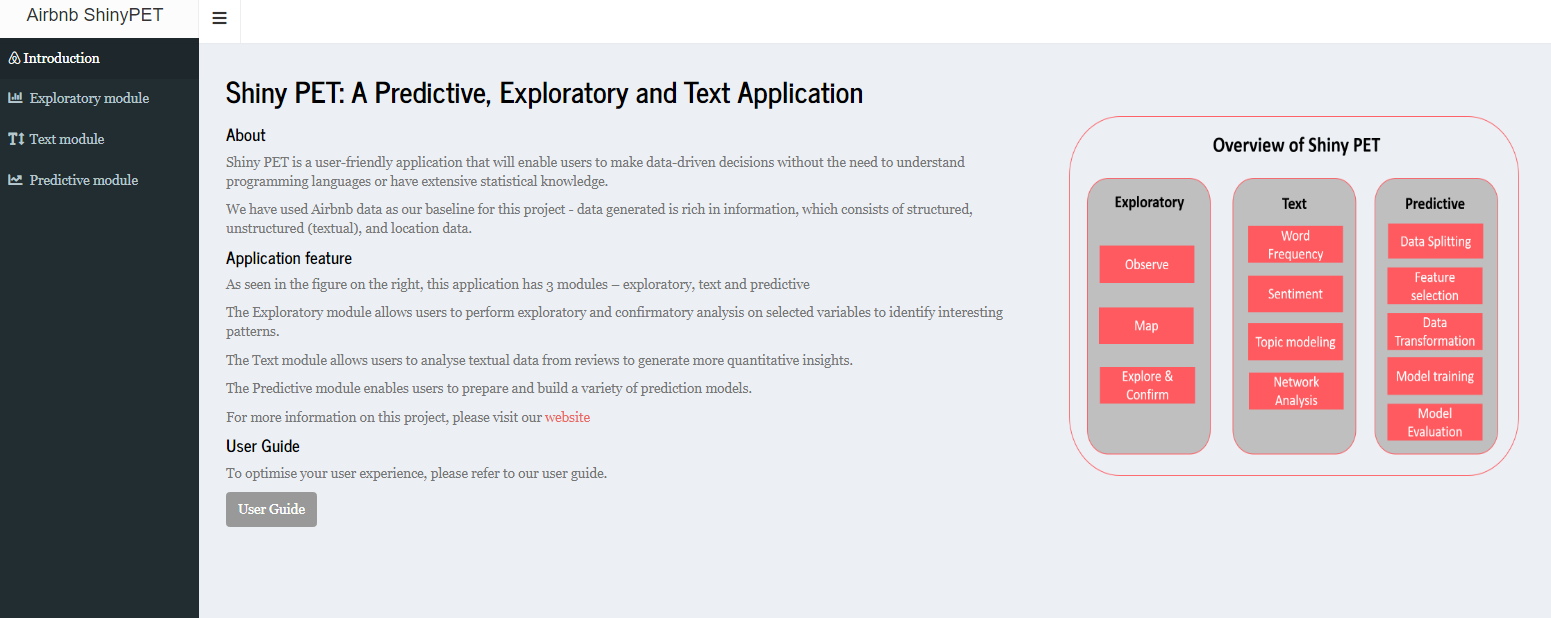
\includegraphics[width=1\linewidth]{images/landing} 

}

\caption{Landing page of Shiny PET}\label{fig:unnamed-chunk-1}
\end{figure}

The landing page of the application provides a brief background for this
application, its features and overview of its navigation.

\hypertarget{exploratory}{%
\subsection{2. Exploratory}\label{exploratory}}

\hypertarget{observe}{%
\subsubsection{2.1 Observe}\label{observe}}

This tab allows user to quickly understand the data to be analysed.

\begin{figure}[H]

{\centering 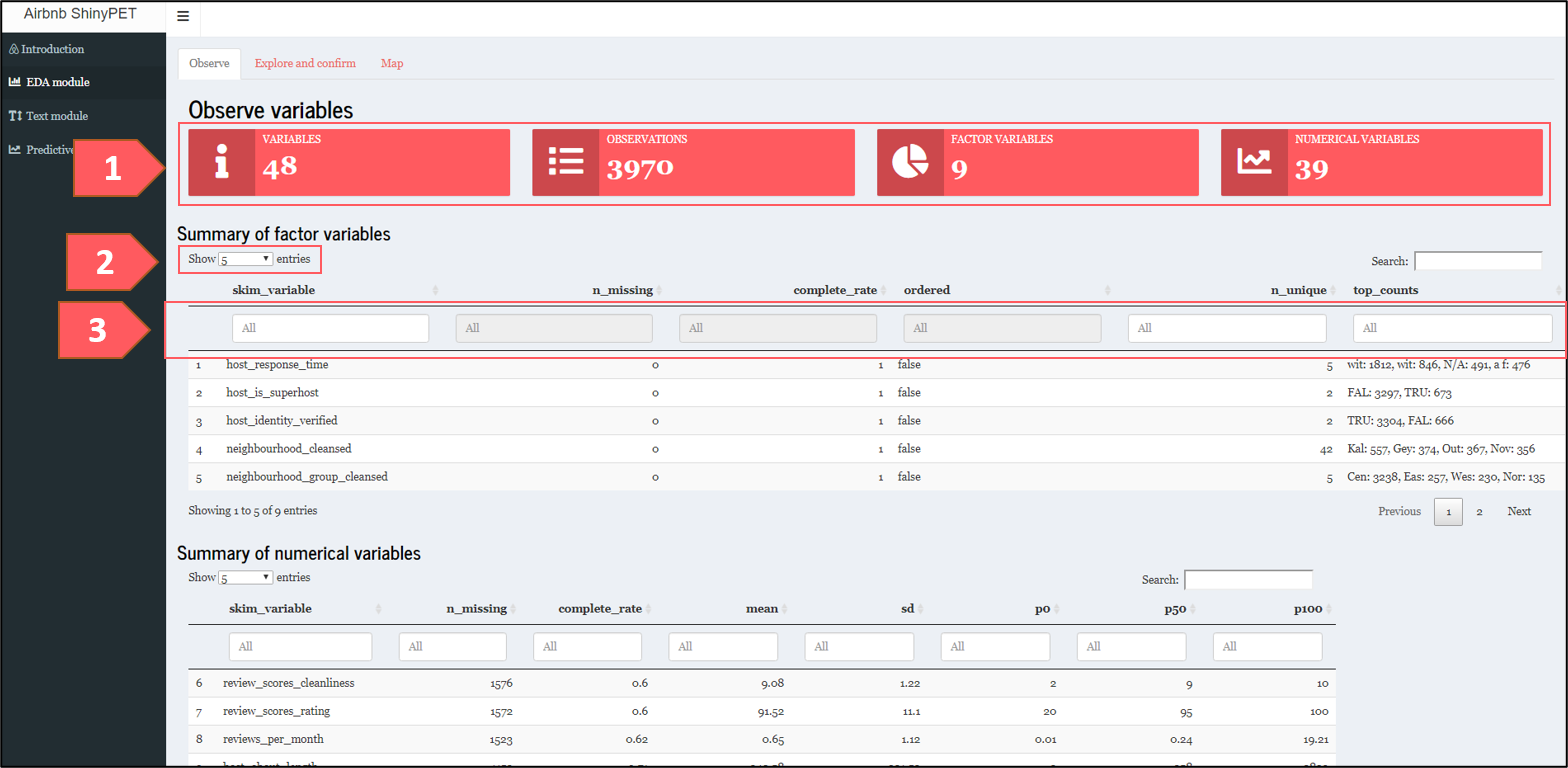
\includegraphics[width=1\linewidth]{images/observe} 

}

\caption{Observe tab of Explore module}\label{fig:unnamed-chunk-2}
\end{figure}

{[}1{]} Shows the summary of data.

{[}2{]} Change number of observations shown. To minimize having to
constantly select ``Next'' to view hidden variables, users can show the
maximum entries (i.e 100) to be displayed.

{[}3{]} Search data if necessary.

\hypertarget{map}{%
\subsubsection{2.2 Map}\label{map}}

This tab allows user to explore the geographic patterns of Airbnb
listings through 2 thematic maps - point symbol and choropleth.

\hypertarget{point-symbol-map}{%
\paragraph{2.2.1 Point Symbol map}\label{point-symbol-map}}

Each point on the map is a listing. This allows user to see how
distributed Airbnbs are throughout Singapore.

\begin{figure}[H]

{\centering 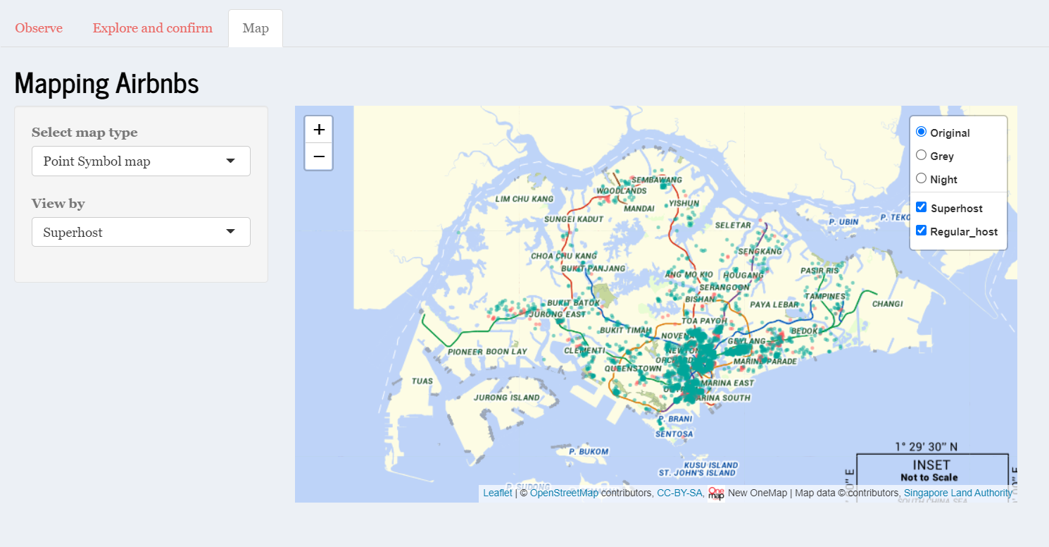
\includegraphics[width=1\linewidth]{images/map} 

}

\caption{Point Symbol Map}\label{fig:unnamed-chunk-3}
\end{figure}

{[}1{]} Select map type. Map will auto update upon selection.

{[}2{]} Select between superhost and room type. This shows the listings
by selected variables.

{[}3{]} Zoom in and out the map.

\begin{figure}[H]

{\centering 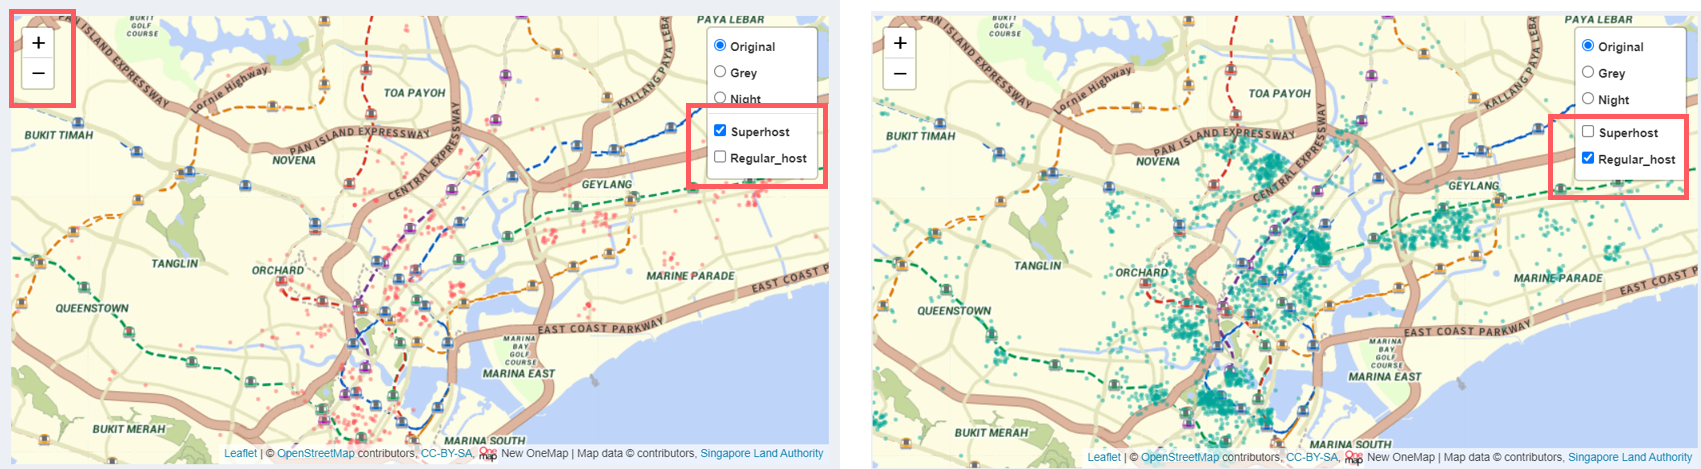
\includegraphics[width=1\linewidth]{images/map1} 

}

\caption{View selected listings}\label{fig:unnamed-chunk-4}
\end{figure}

{[}4{]} User can check and uncheck to view selected listings.

\begin{figure}[H]

{\centering 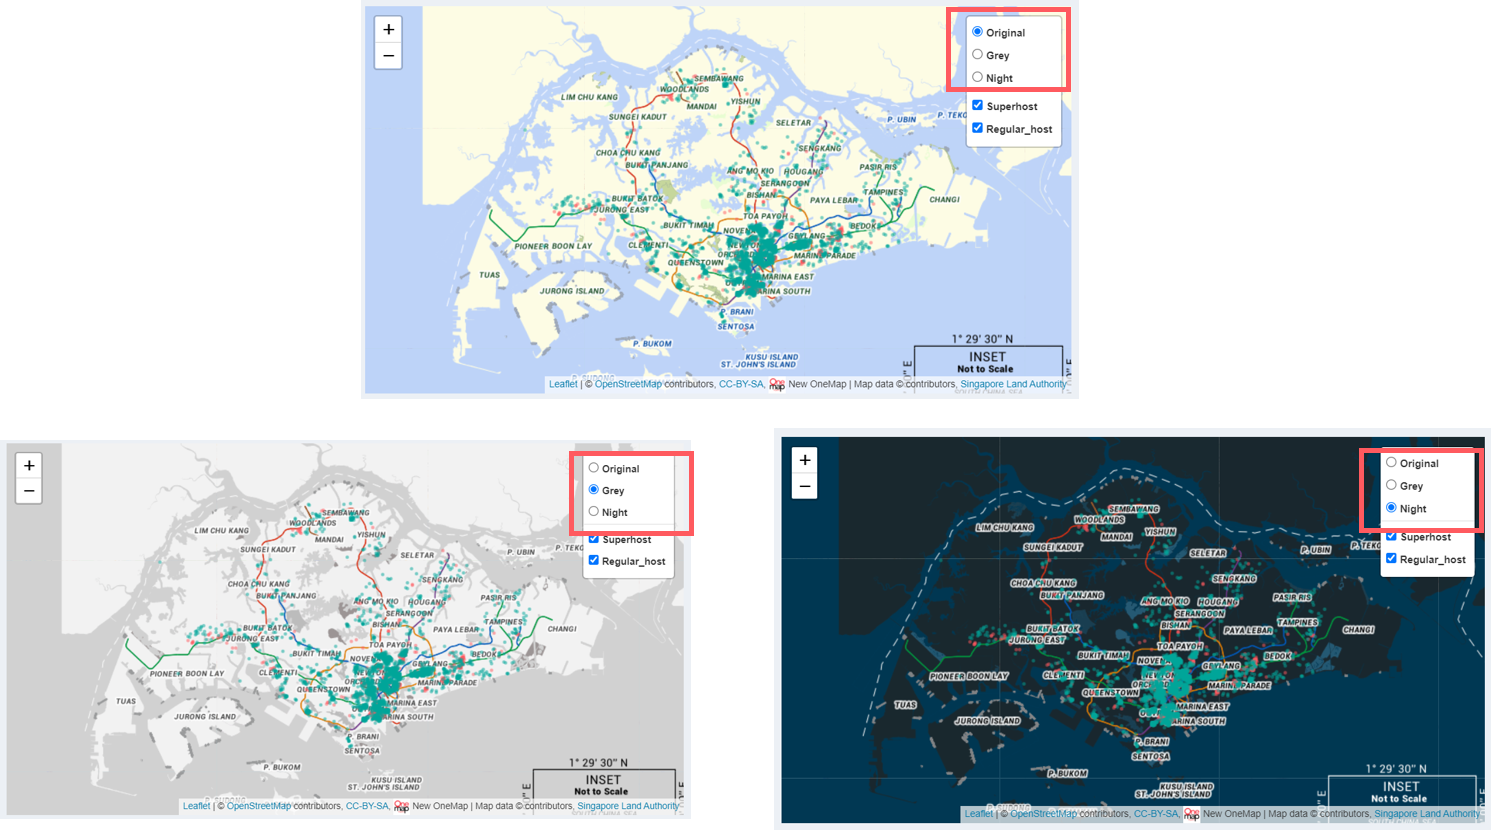
\includegraphics[width=1\linewidth]{images/background} 

}

\caption{3 types of background colour}\label{fig:unnamed-chunk-5}
\end{figure}

{[}5{]} User can select between different background.

\hypertarget{choropleth-map}{%
\paragraph{2.2.1 Choropleth map}\label{choropleth-map}}

\begin{figure}[H]

{\centering 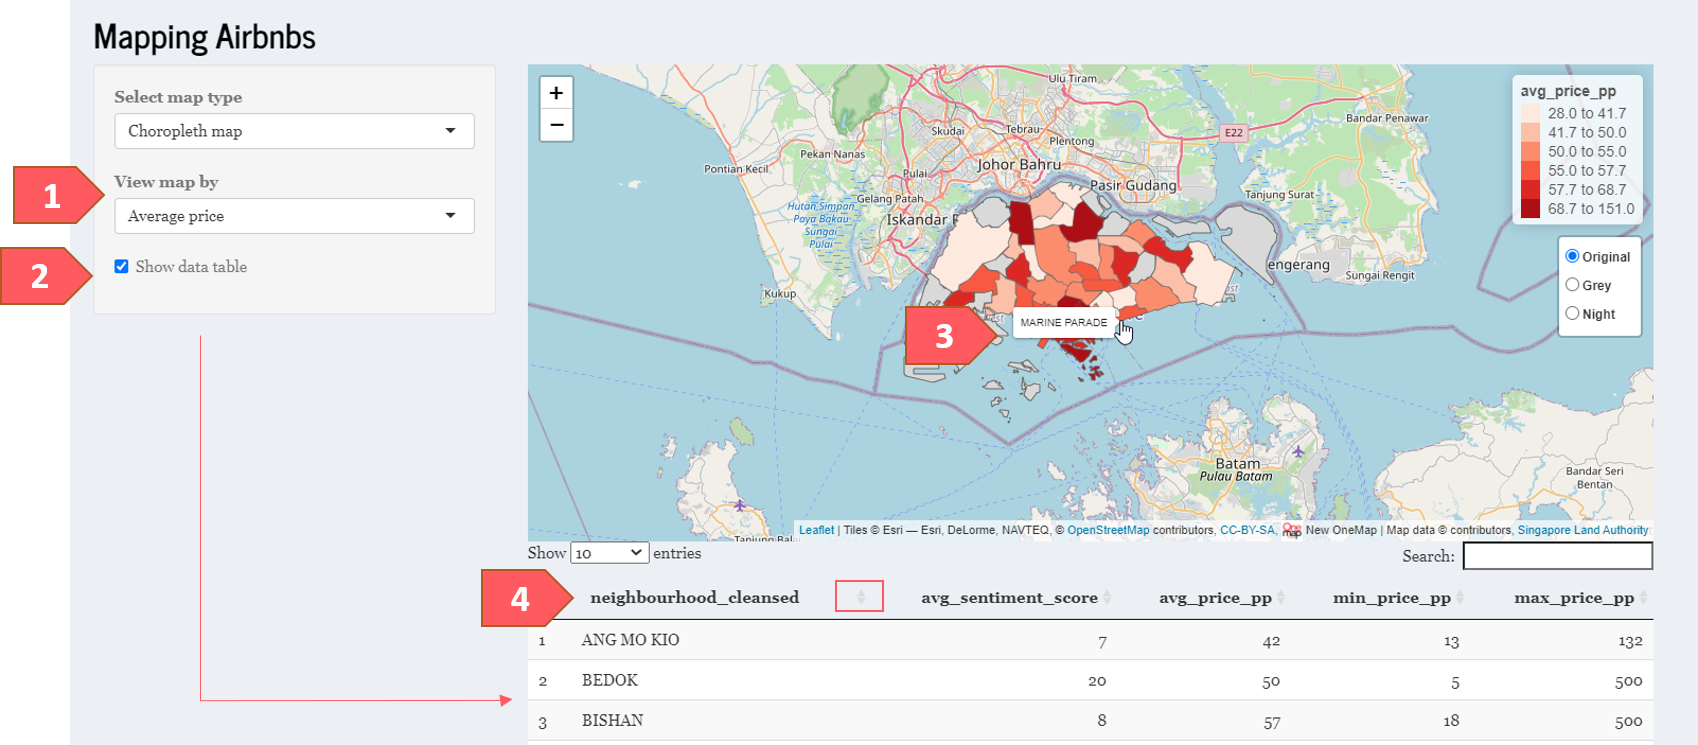
\includegraphics[width=1\linewidth]{images/choro} 

}

\caption{Choropleth map}\label{fig:unnamed-chunk-6}
\end{figure}

{[}1{]} Select between average price and average sentiment score. The
average sentiment score is calculated based on the positive and negative
of guests' reviews. For more details on sentiment of reviews, please fer
to the Text module \textgreater{} Sentiment Analysis tab.

{[}2{]} User can decide whether to view the data by checking /
unchecking the `Show data table' box.

{[}3{]} Hover over the area to see neighbourhood names.

{[}4{]} User can sort table according to needs.

\hypertarget{explore-and-confirm}{%
\subsubsection{2.3 Explore and Confirm}\label{explore-and-confirm}}

This tab allows users to perform exploratory and confirmatory analysis.

\hypertarget{types-of-chart-available}{%
\paragraph{2.3.1 Types of chart
available}\label{types-of-chart-available}}

User can explore the dataset using different charts.

\begin{figure}[H]

{\centering 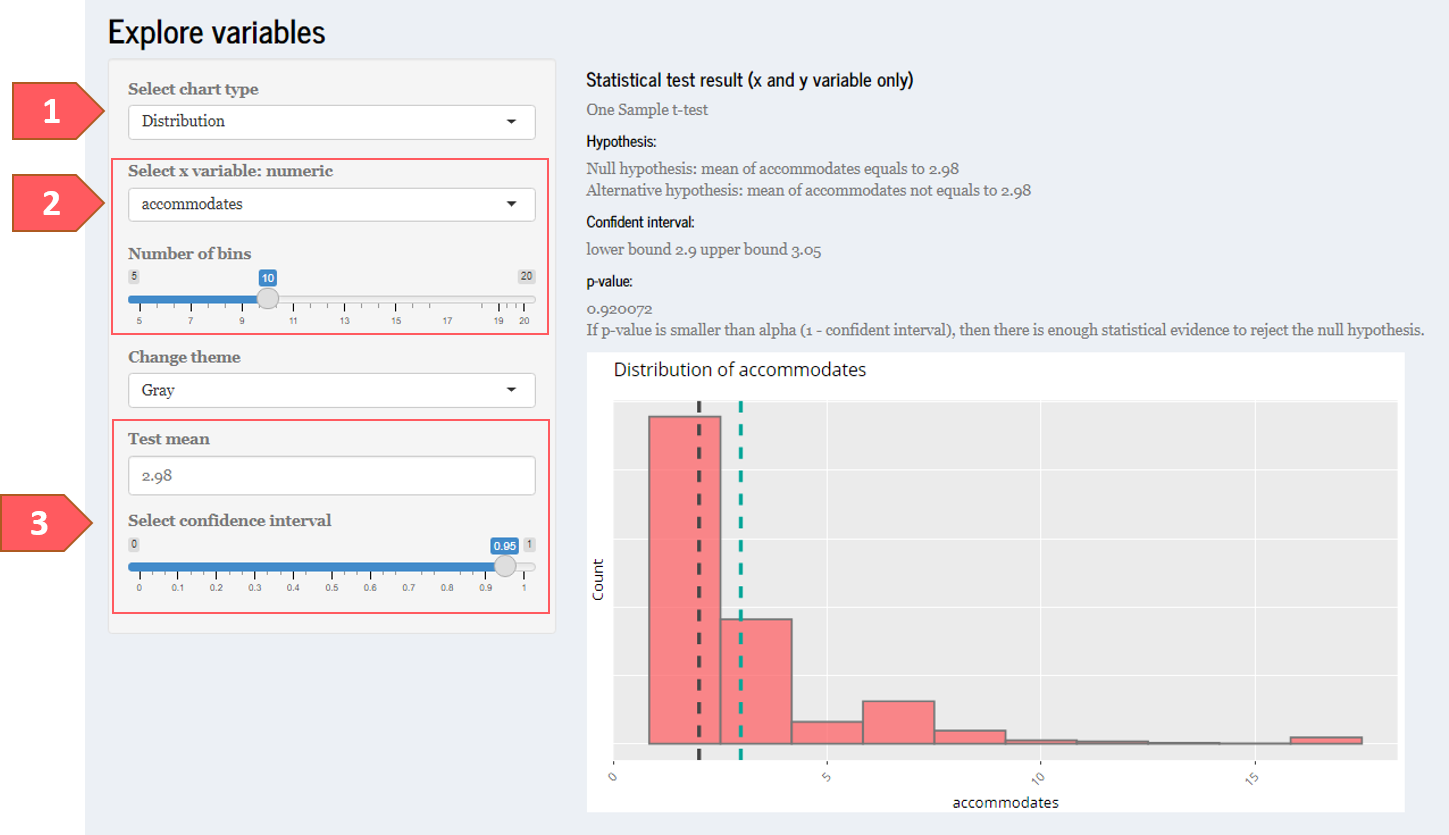
\includegraphics[width=0.95\linewidth]{images/explore2} 

}

\caption{Explore and Confirm tab of Explore module}\label{fig:unnamed-chunk-7}
\end{figure}

{[}1{]} There are 4 types of chart:

\begin{figure}[H]

{\centering 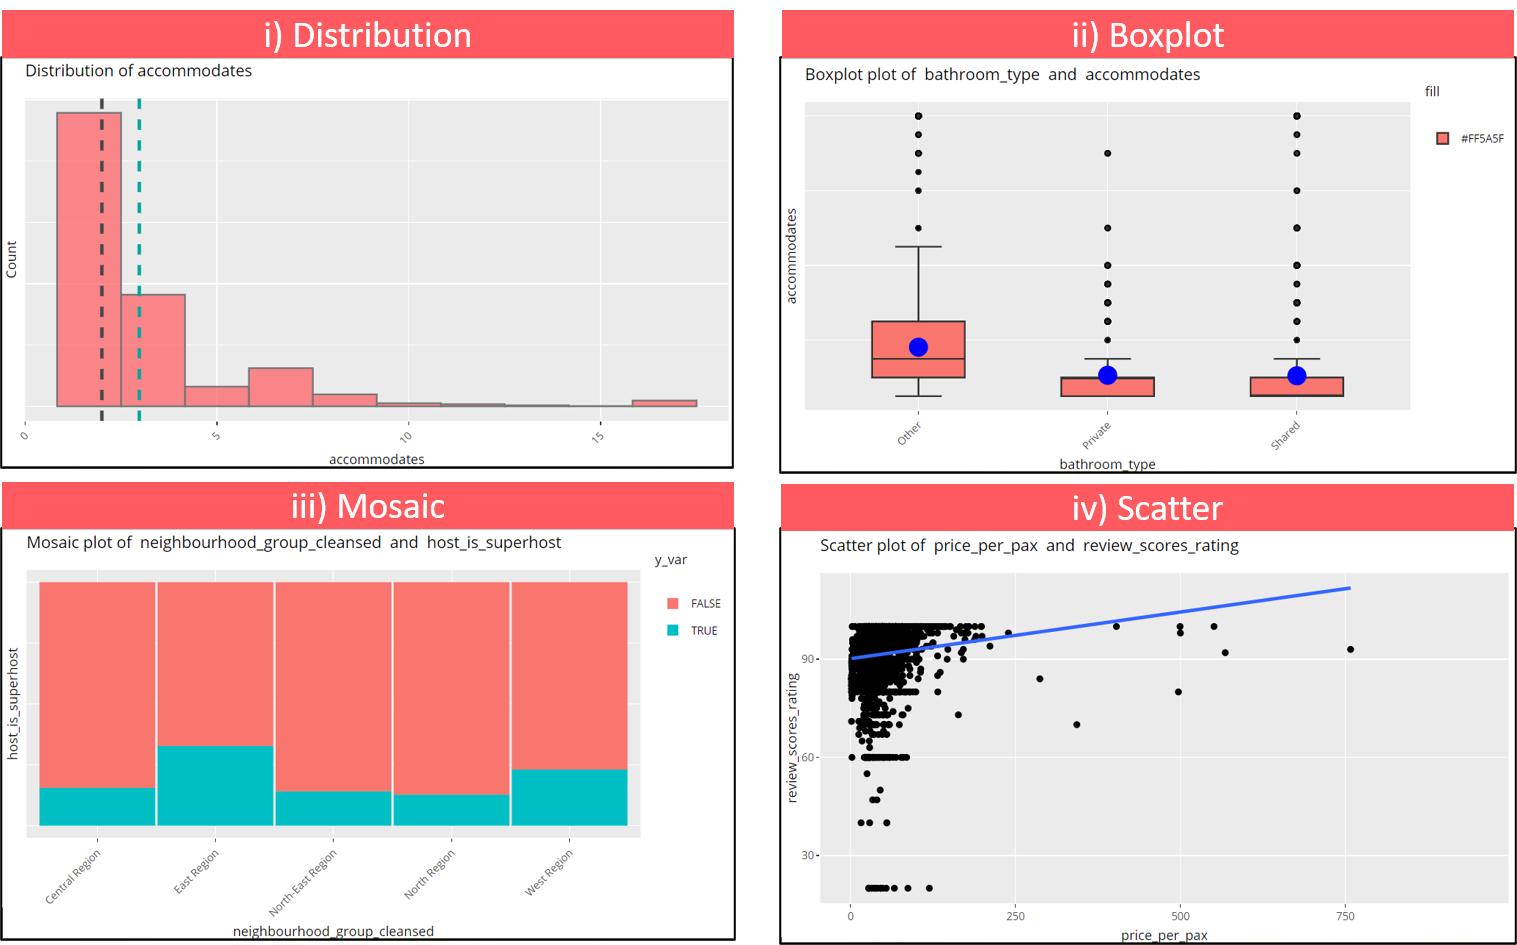
\includegraphics[width=0.8\linewidth]{images/plots} 

}

\caption{Four types of charts available}\label{fig:unnamed-chunk-8}
\end{figure}

\begin{enumerate}
\def\labelenumi{\roman{enumi})}
\tightlist
\item
  Distribution - to analyse a single variable (univariate analysis).
\end{enumerate}

\begin{itemize}
\tightlist
\item
  teal line refers to mean\\
\item
  black line refers to median
\end{itemize}

\begin{enumerate}
\def\labelenumi{\roman{enumi})}
\setcounter{enumi}{1}
\tightlist
\item
  Boxplot - to analyse 1 factor and 1 numeric variables
\end{enumerate}

\begin{itemize}
\tightlist
\item
  Blue cirlce refers to mean
\end{itemize}

\begin{enumerate}
\def\labelenumi{\roman{enumi})}
\setcounter{enumi}{2}
\item
  Mosaic - to analyse two factor variables
\item
  Scatter - to analyse two numeric variables
\end{enumerate}

{[}2{]} Selection available will change according to chart type.

{[}3{]} Statistical test options available will change according to
chart type.

\hypertarget{performing-exploratory-and-confirmatory-analysis}{%
\paragraph{2.3.2 Performing exploratory and confirmatory
analysis}\label{performing-exploratory-and-confirmatory-analysis}}

\begin{figure}[H]

{\centering 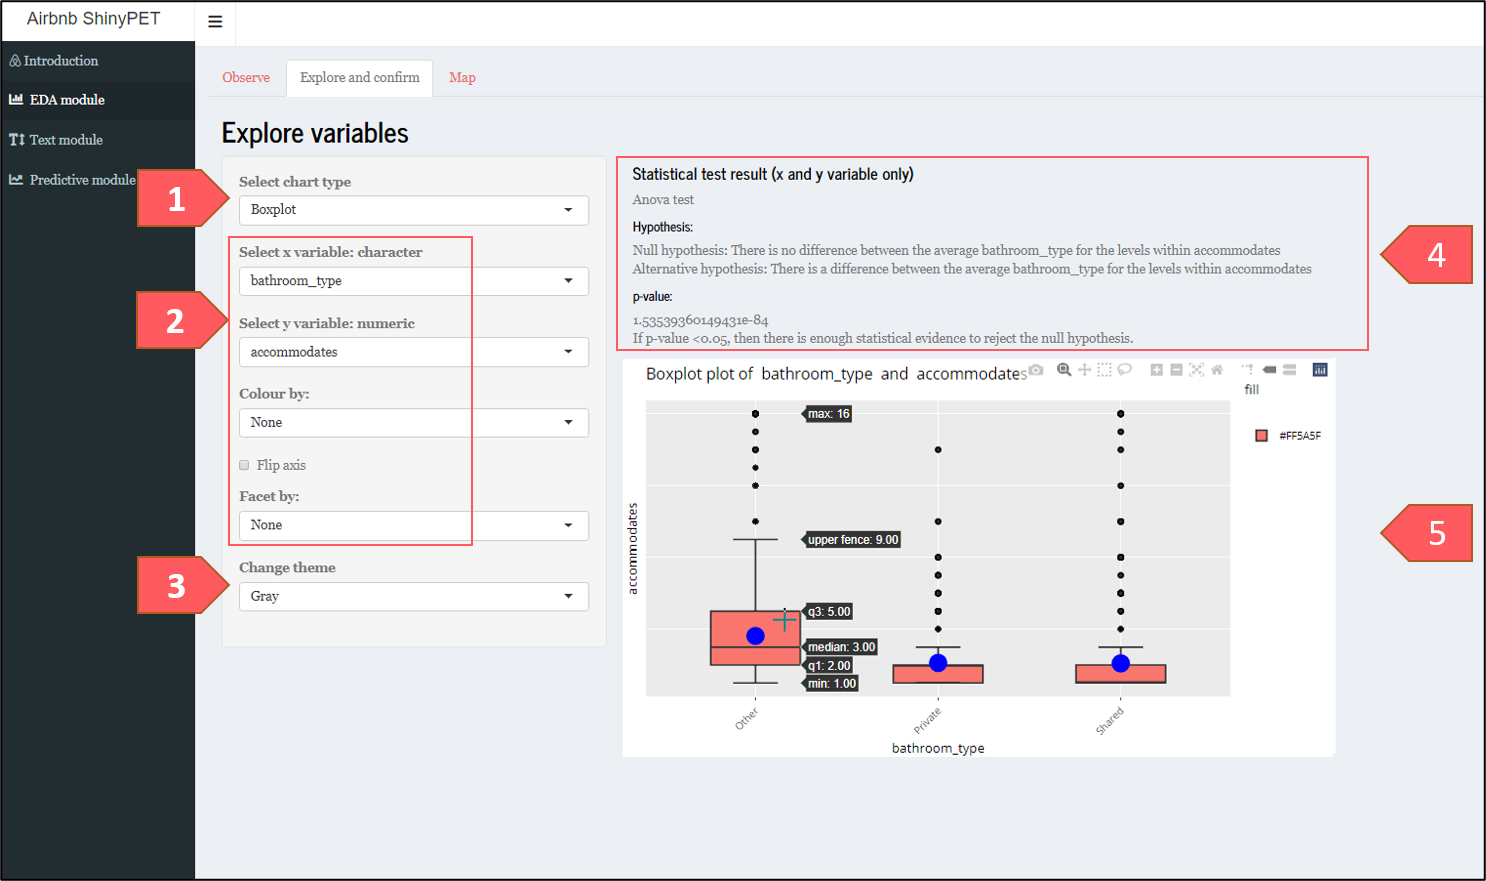
\includegraphics[width=1\linewidth]{images/explore1} 

}

\caption{Explore and Confirm tab of Explore module}\label{fig:unnamed-chunk-9}
\end{figure}

{[}1{]} Select chart type.

{[}2{]} Select the variables that you are interested in analysing.

{[}3{]} This changes the background of the graph.

{[}4{]} The type of statistical tests are automated based on user's x
and y variables. Simply select the variables you wish to analyse.

If p-value is less than the alpha (1 - confident interval), you reject
the null hypothesis and accept the alternative hypothesis.

\textbf{Note:} Statistical test is only applicable to selected x and y
variable, and does not take colour and facet variables into
consideration.

{[}5{]} The chart is interactive and users hover to select a single
object in a plot, highlight selected records by clicking and unclicking
legend, define a region and download the chart.

\begin{figure}[H]

{\centering 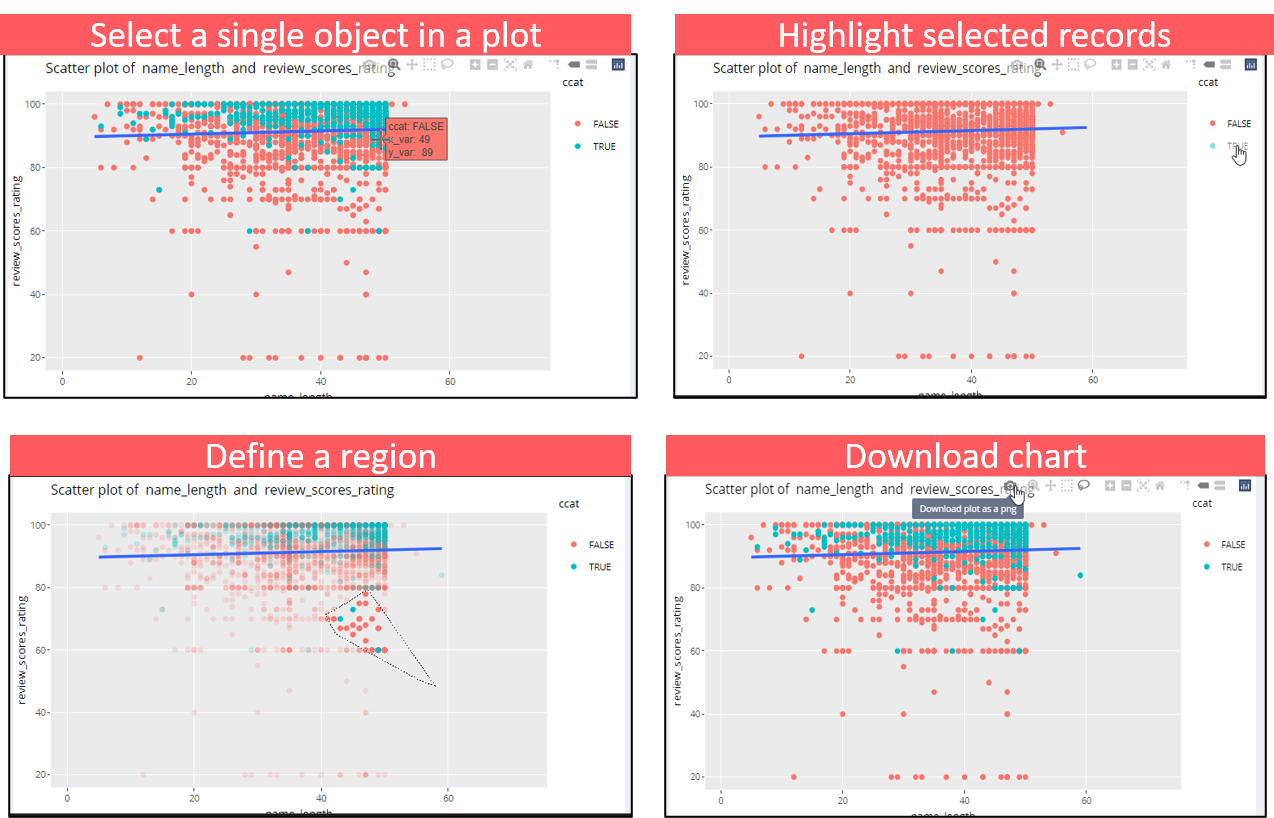
\includegraphics[width=1\linewidth]{images/explore3} 

}

\caption{Interactive chart}\label{fig:unnamed-chunk-10}
\end{figure}

\hypertarget{text}{%
\subsection{3. Text}\label{text}}

\hypertarget{word-cloud}{%
\subsubsection{3.1 Word Cloud}\label{word-cloud}}

There are two charts shown.

\begin{figure}[H]

{\centering 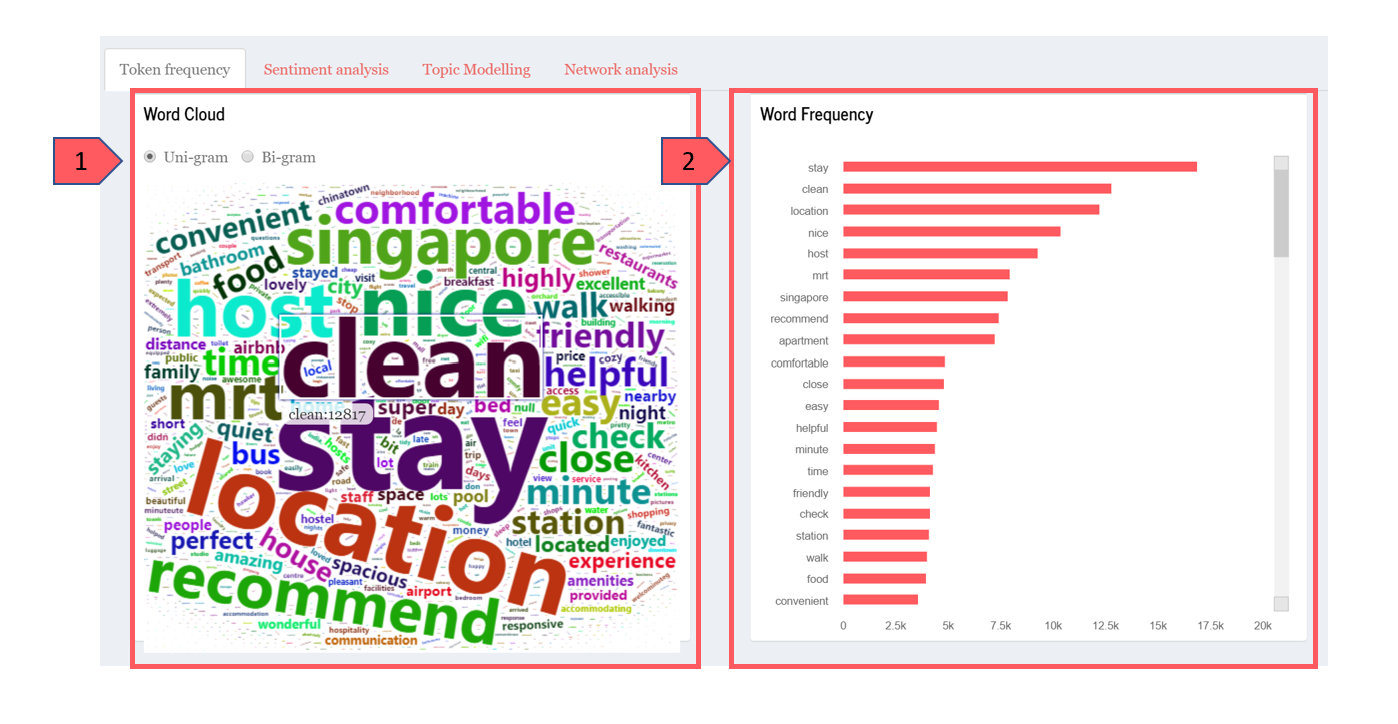
\includegraphics[width=0.95\linewidth]{images/wordcloud} 

}

\caption{Uni-gram}\label{fig:unnamed-chunk-11}
\end{figure}

{[}1{]} Word cloud.

{[}2{]} Frequency Bar Chart.

\begin{figure}[H]

{\centering 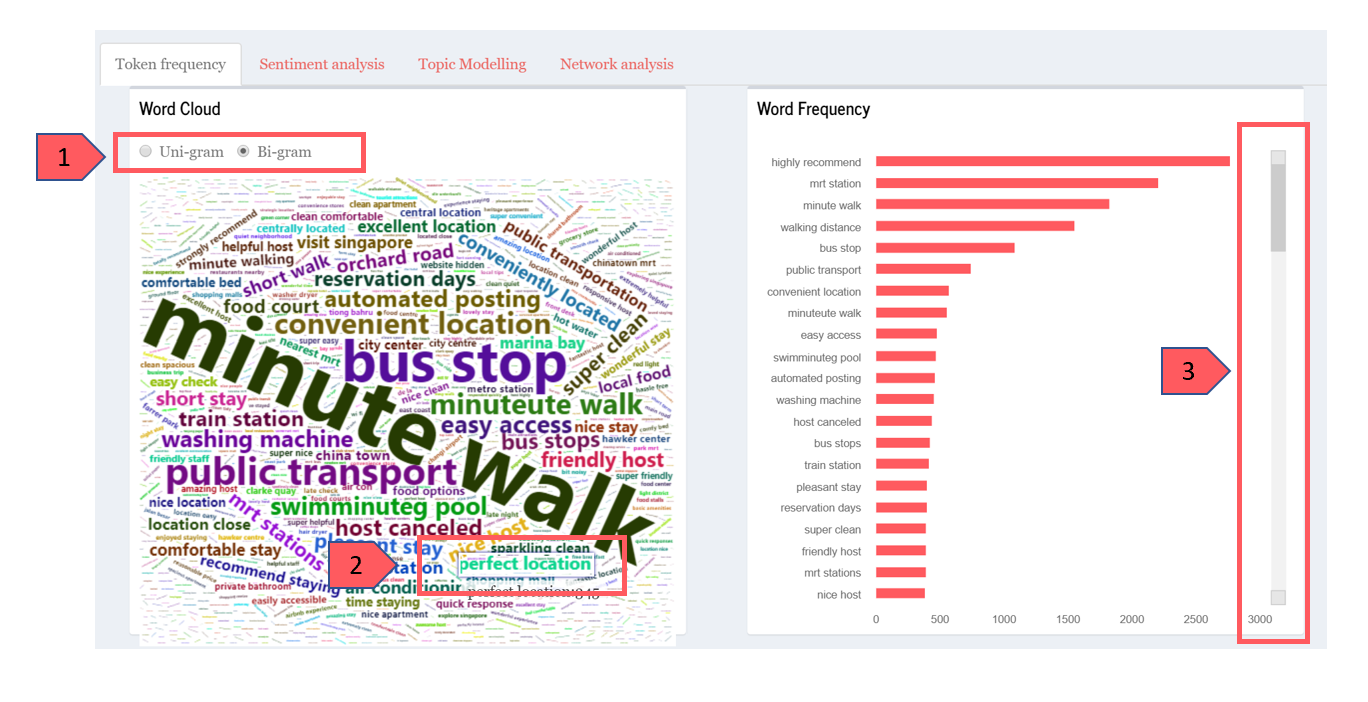
\includegraphics[width=0.95\linewidth]{images/wordcloud2} 

}

\caption{Bi-gram}\label{fig:unnamed-chunk-12}
\end{figure}

{[}1{]} Select chart type - Unigram or Bigram.

{[}2{]} Hover over each word to observe it frequency.

{[}3{]} Scroll up/down to see the occurrence of words in a descending
order.

\hypertarget{sentiment-analysis}{%
\subsubsection{3.2 Sentiment Analysis}\label{sentiment-analysis}}

There are two charts shown.

\begin{figure}[H]

{\centering 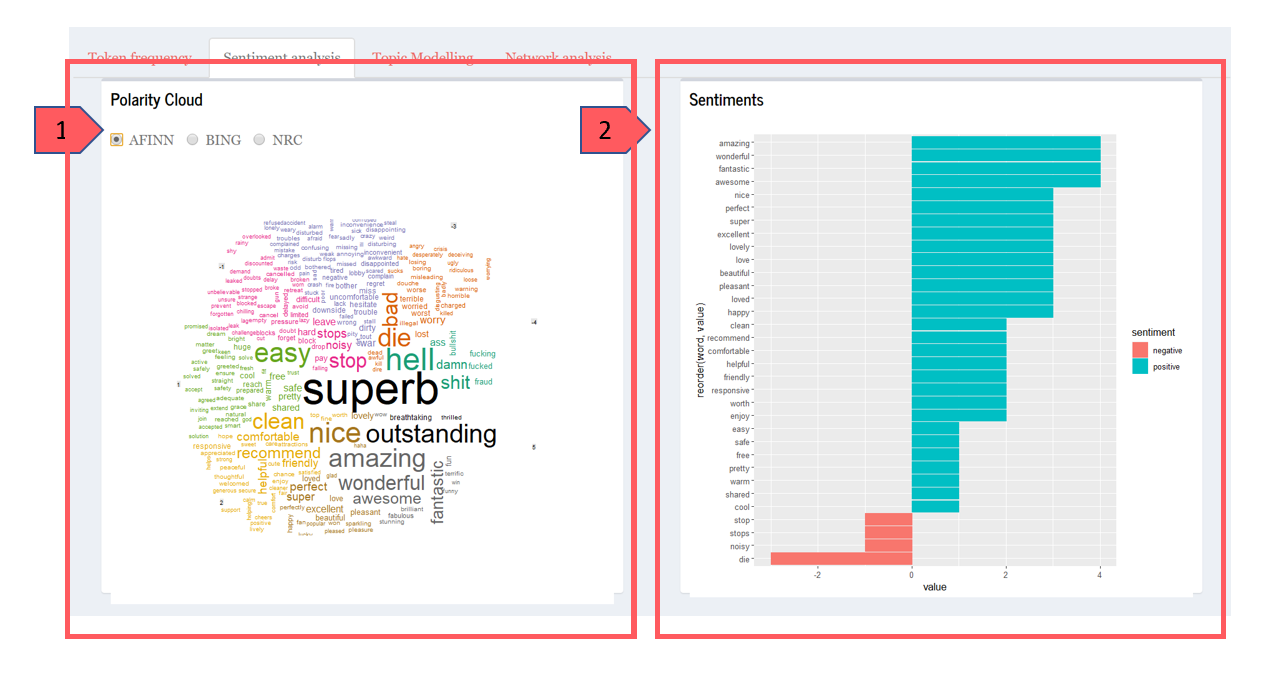
\includegraphics[width=0.95\linewidth]{images/sentimentchart} 

}

\caption{AFINN}\label{fig:unnamed-chunk-13}
\end{figure}

{[}1{]} Sentiment Polarity Cloud

{[}2{]} Bar Chart/Radial Plot

\begin{figure}[H]

{\centering 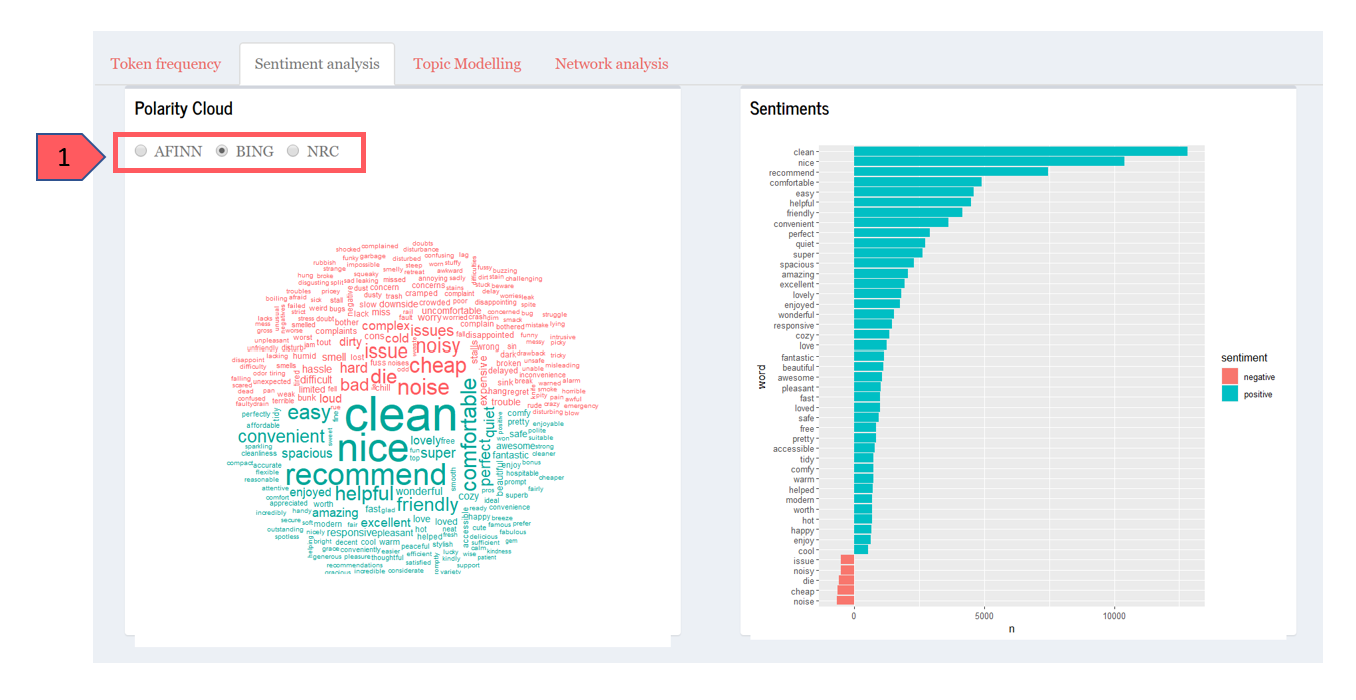
\includegraphics[width=0.95\linewidth]{images/bingchart} 

}

\caption{BING}\label{fig:unnamed-chunk-14}
\end{figure}

\begin{figure}[H]

{\centering 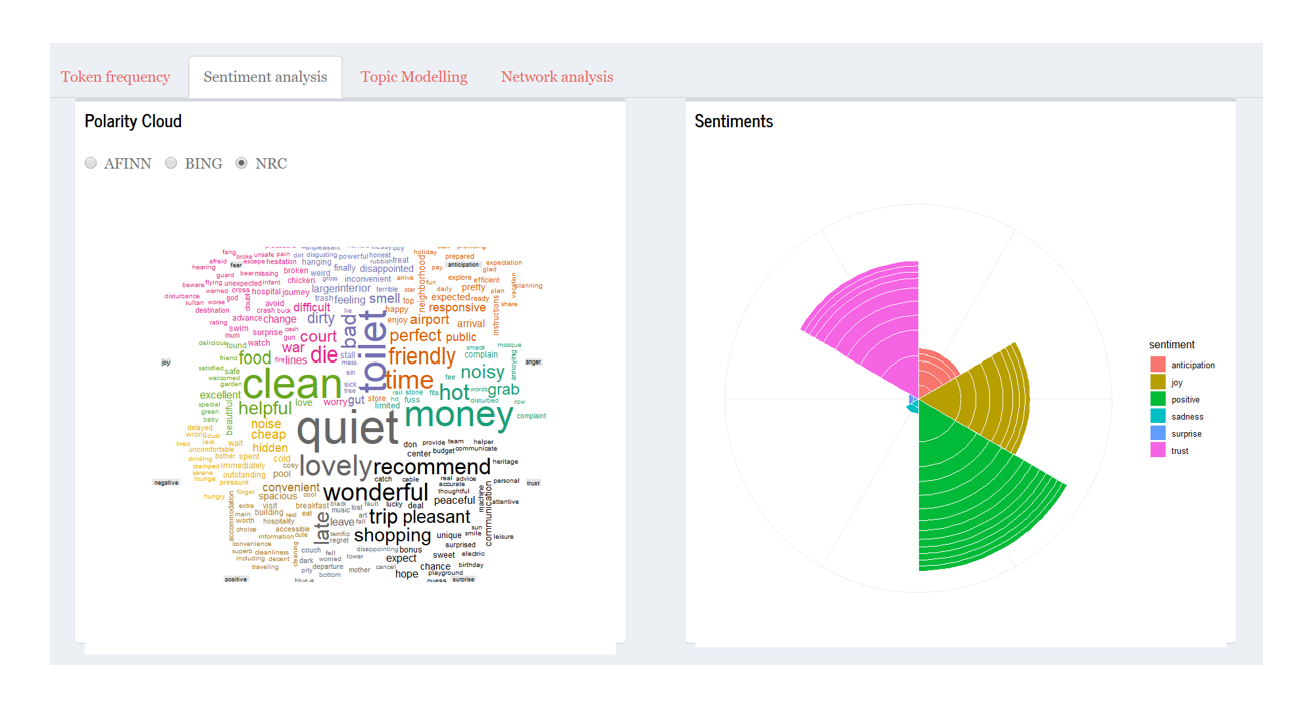
\includegraphics[width=0.95\linewidth]{images/nrcchart} 

}

\caption{NRC}\label{fig:unnamed-chunk-15}
\end{figure}

{[}1{]} Select lexicon - AFINN, BING or NRC.

{[}2{]} AFINN cloud word cloud with 5 different values in different
colours and the related bar chart will show the value and frequency of
occurrence of each word, in a descending order

{[}3{]} BING cloud will show positive and negative sentiments in blue
and red colour respectively with the related bar chart showing the value
and frequency of occurrence of each word, in a descending order

{[}4{]} NRC cloud will show words with 8 different emotions and 2
sentiments. The radial plot illustrates the frequency of words
appearing.

\hypertarget{topic-modelling}{%
\subsubsection{3.3 Topic Modelling}\label{topic-modelling}}

\begin{figure}[H]

{\centering 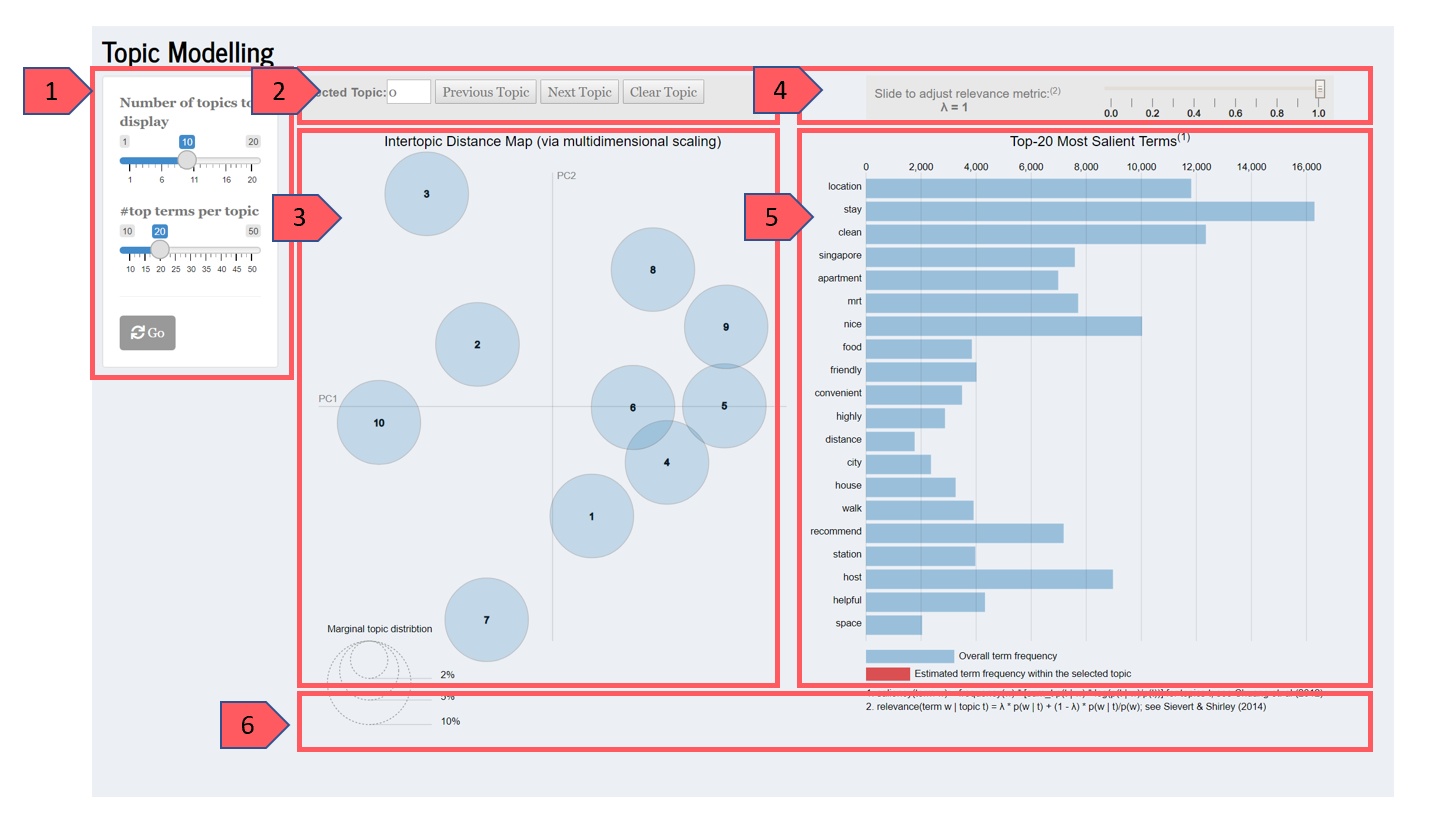
\includegraphics[width=0.95\linewidth]{images/topicmodelling} 

}

\caption{Topic Modelling}\label{fig:unnamed-chunk-16}
\end{figure}

{[}1{]} Slide number of topics to display, top terms per topic, then
press ``Go''.

{[}2{]} After the graph is plotted, type the topic.

{[}3{]} Intertopic Distance Map will be shown.

{[}4{]} Slide to adjust relevance metric.

{[}5{]} Bar chart of top 20 most salient terms will be shown.

{[}6{]} Brief explanation of relevancy and saliency are described in the
footnote.

\hypertarget{network-analysis}{%
\subsubsection{3.4 Network Analysis}\label{network-analysis}}

\begin{figure}[H]

{\centering 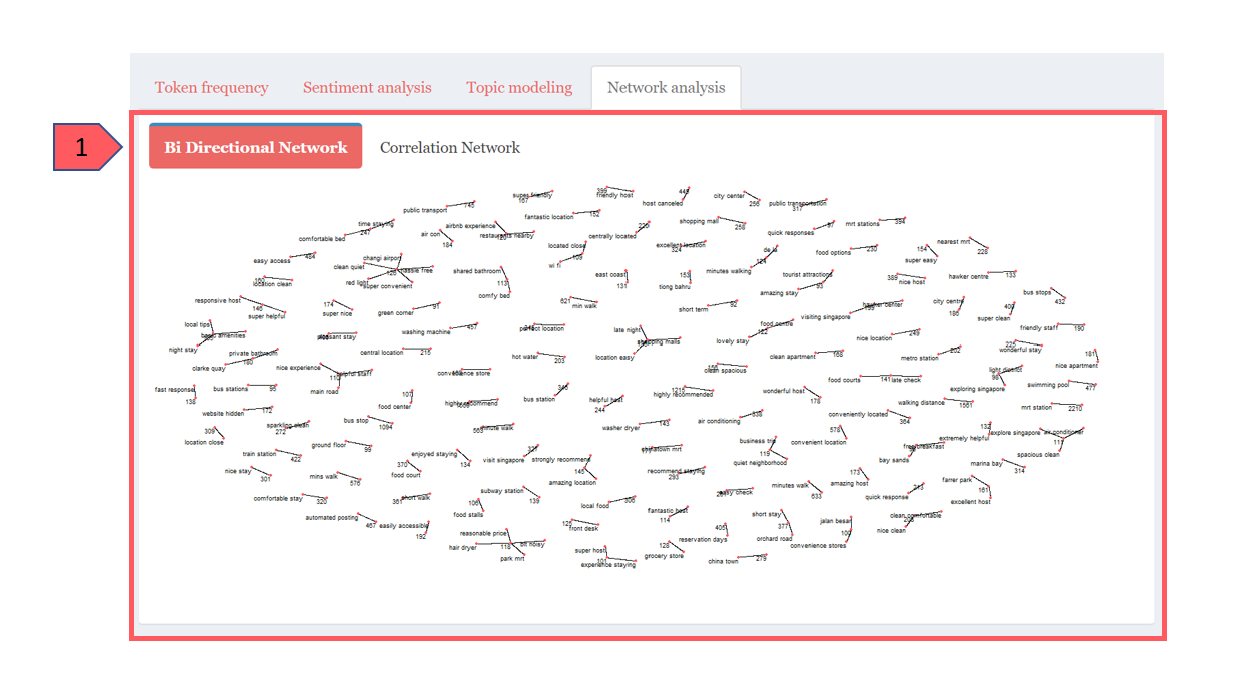
\includegraphics[width=0.95\linewidth]{images/network} 

}

\caption{Network Analysis}\label{fig:unnamed-chunk-17}
\end{figure}

{[}1{]} Pills button to allow user to observe bi directional or
correlation network.

\hypertarget{predictive}{%
\subsection{4. Predictive}\label{predictive}}

\hypertarget{data-splitting}{%
\subsubsection{4.1 Data splitting}\label{data-splitting}}

The module starts with the tab which allows user to:

{[}1{]} Select the response variable for prediction

{[}2{]} Choose the proportion of training and validation (test) set

{[}3{]} Proceed with data splitting

\begin{figure}[H]

{\centering 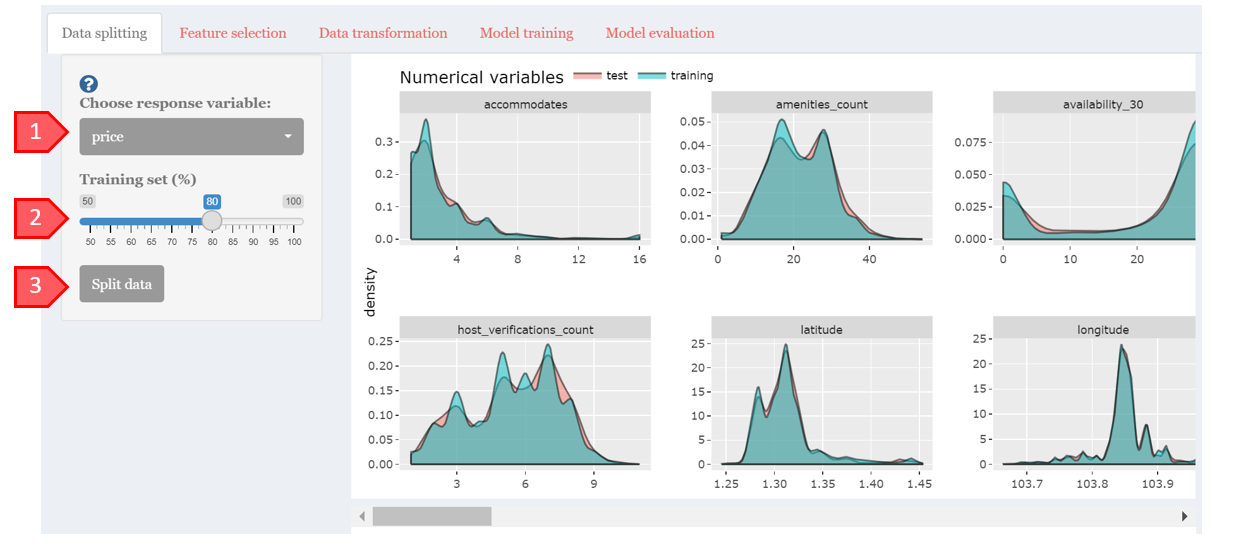
\includegraphics[width=0.95\linewidth]{images/datasplit1} 

}

\caption{Data split tab of Predictive module}\label{fig:unnamed-chunk-18}
\end{figure}

This will then create density plot for numerical variables {[}4{]} and
bar chart for categorical variables {[}5{]} with division between
training and test set.

\begin{figure}[H]

{\centering 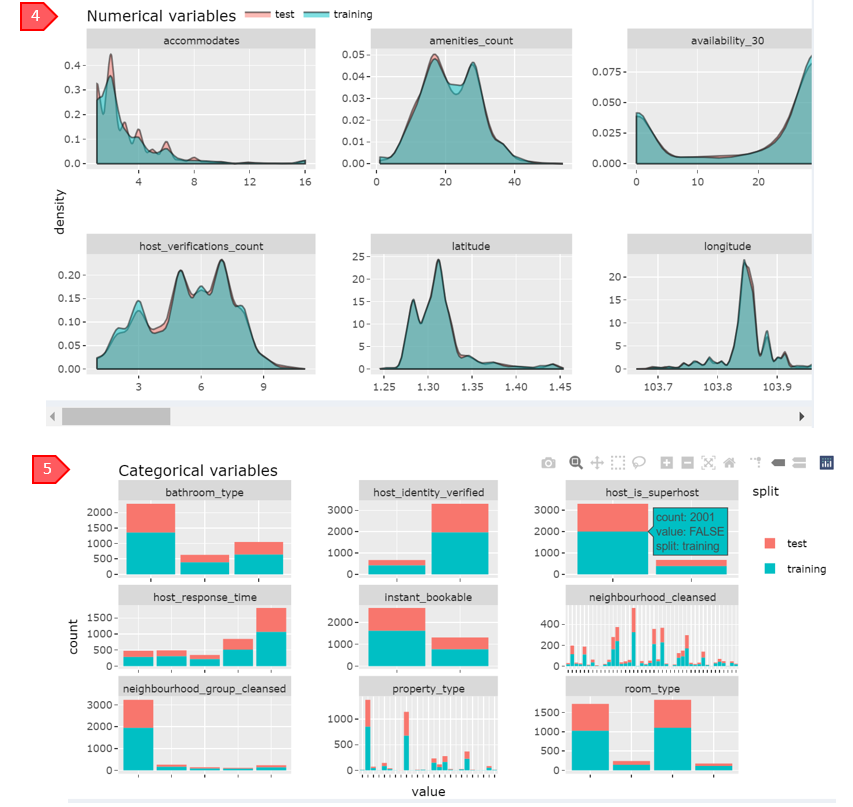
\includegraphics[width=0.95\linewidth]{images/datasplit2} 

}

\caption{Train-test split distribution plot}\label{fig:unnamed-chunk-19}
\end{figure}

\hypertarget{feature-selection}{%
\subsubsection{4.2 Feature selection}\label{feature-selection}}

User will be presented with 2 options for feature selection process:
correlation matrix and feature selection using Random Forest and Boruta
method. In the correlation matrix section, user can:

{[}1{]} Select variables of choice

{[}2{]} Select correlation method

{[}3{]} Select p-value significance criteria

{[}4{]} Produce correlation matrix

{[}5{]} Hover over matrix to view details on correlation value and
p-value

\begin{figure}[H]

{\centering 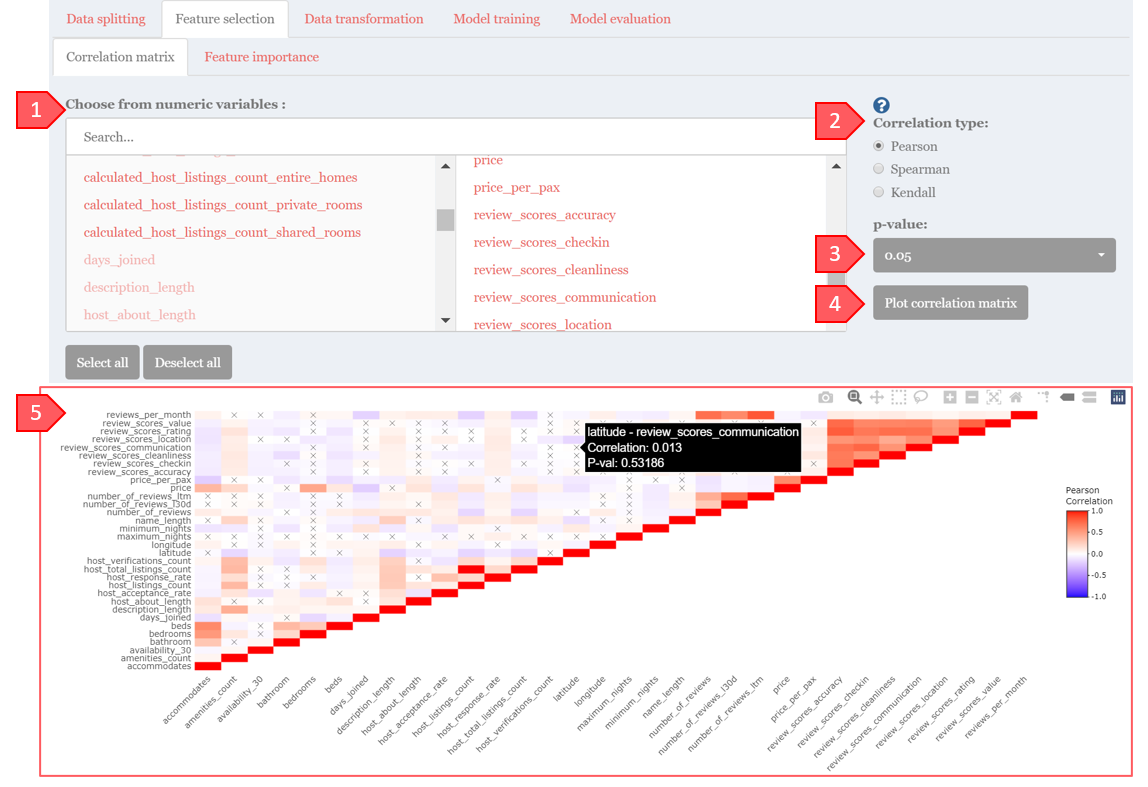
\includegraphics[width=0.95\linewidth]{images/corrmatrix} 

}

\caption{Correlation matrix tab of feature selection}\label{fig:unnamed-chunk-20}
\end{figure}

In the next section, user may decide to run the feature selection
process by Random Forest and Boruta method using the training set
created from the previous data splitting section. The plot for both
methods will be displayed side by side for comparison.

\begin{figure}[H]

{\centering 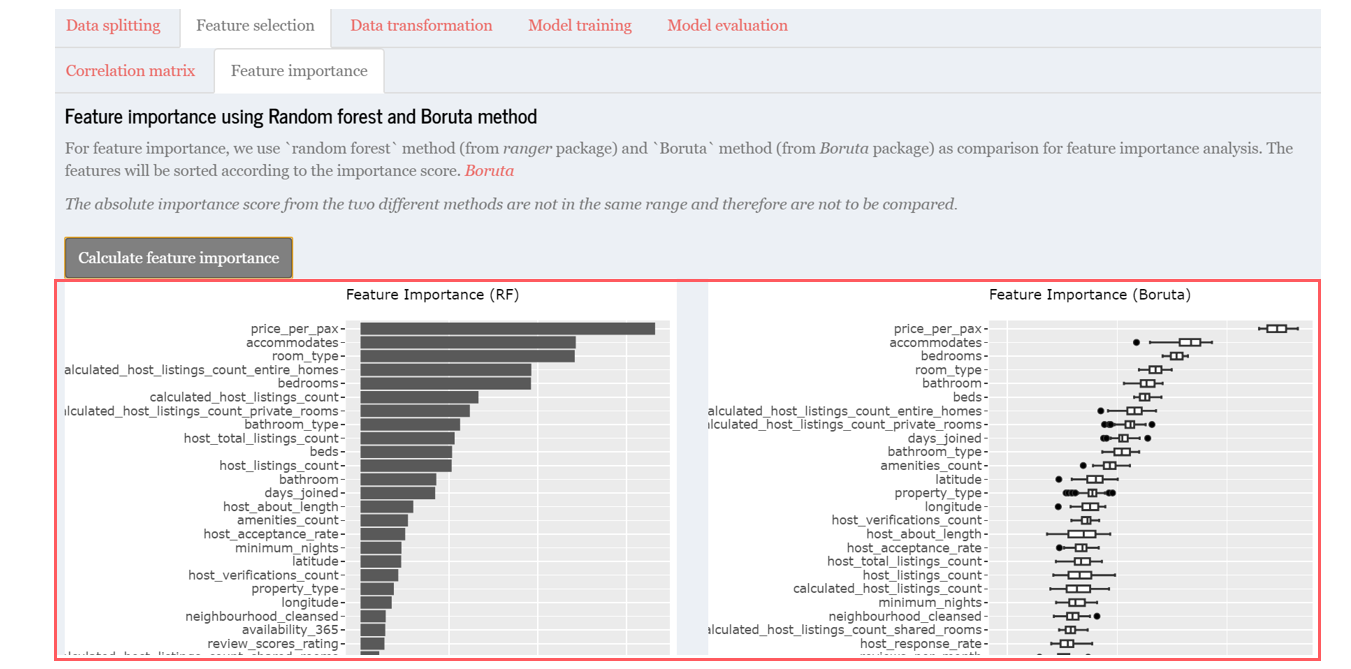
\includegraphics[width=0.95\linewidth]{images/featureselect} 

}

\caption{Feature selection tab comparing 2 different methods}\label{fig:unnamed-chunk-21}
\end{figure}

\hypertarget{variables-and-recipe}{%
\subsubsection{4.3 Variables and recipe}\label{variables-and-recipe}}

Based on the result in the feature selection section, this tab allow
user to filter the variables to be included in the predictive model.
This can be done through the multi-input selection form {[}1{]}. This
module comes with predefined data transformation steps which can be
displayed by clicking on the ``Prepare recipe'' button {[}2{]}. This
will provide user with the recipes that will be executed in data
transformation prior to model training {[}3{]}. To finalise variable
selections and apply the transformation steps, user can click on the
``Transform variables'' button {[}4{]} which will navigate the page to
the next section.

\begin{figure}[H]

{\centering 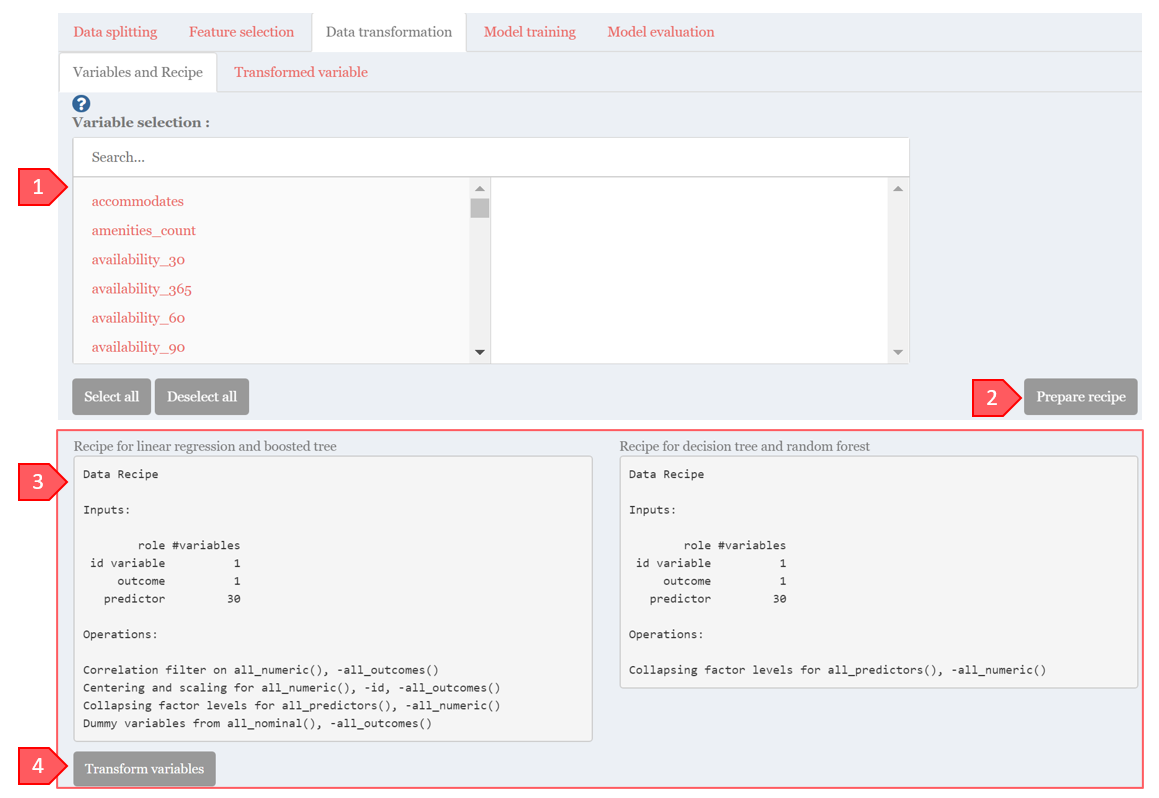
\includegraphics[width=0.95\linewidth]{images/datatrf1} 

}

\caption{Variable selection and data transformation tab}\label{fig:unnamed-chunk-22}
\end{figure}

In this section, user will be able to check the train-test split
distribution once again after variable selection.

\begin{figure}[H]

{\centering 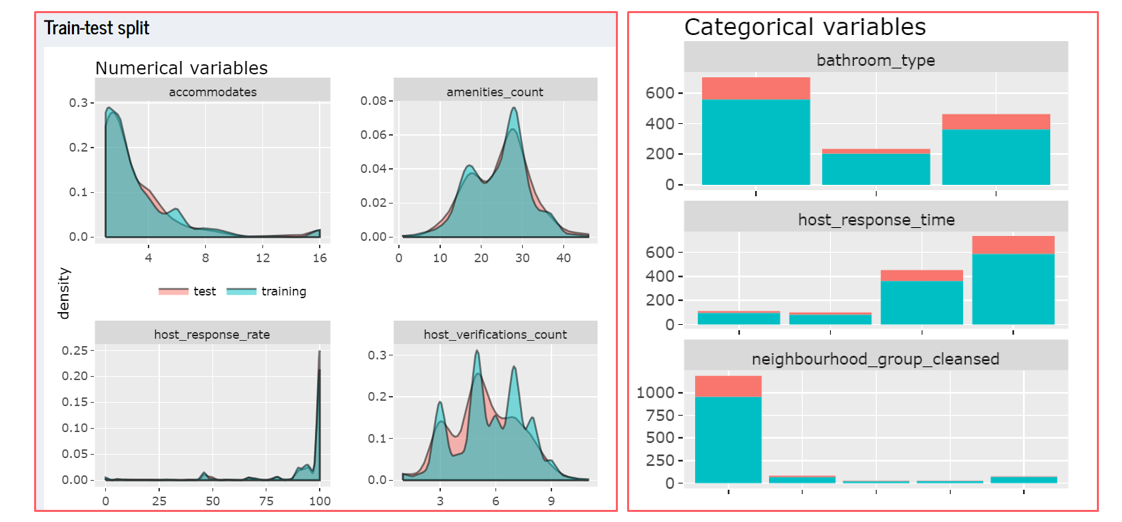
\includegraphics[width=0.95\linewidth]{images/datatrf2} 

}

\caption{Train-test split distribution after variable selection}\label{fig:unnamed-chunk-23}
\end{figure}

The transformed numerical variables are also displayed for comparison,
with option to select variable of interest {[}5{]}.

\begin{figure}[H]

{\centering 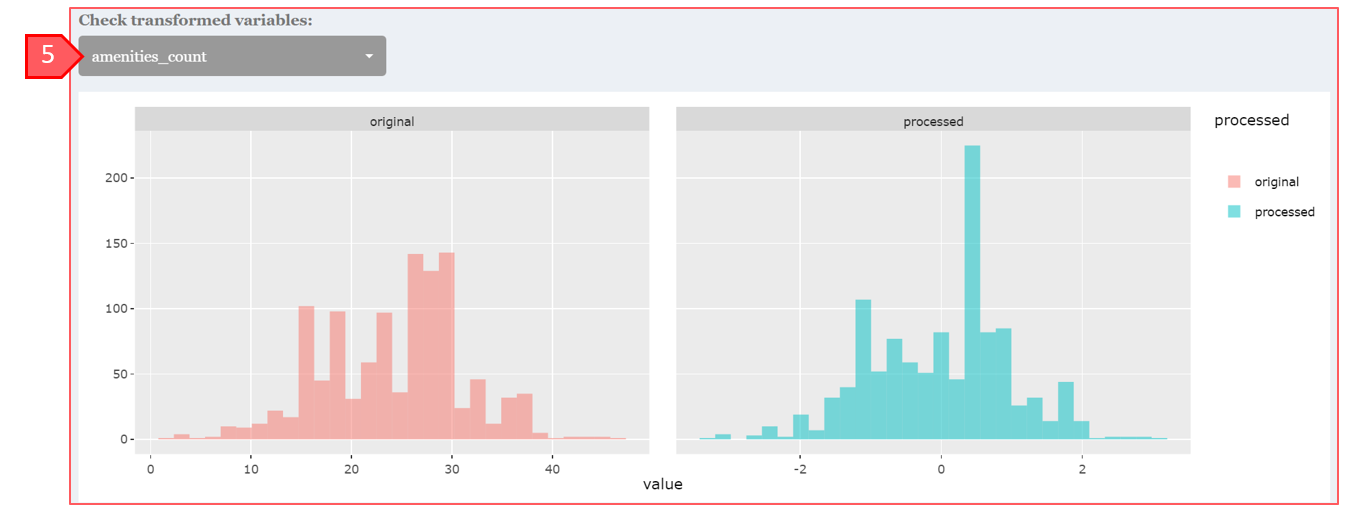
\includegraphics[width=0.95\linewidth]{images/datatrf3} 

}

\caption{Transformed variables before and after comparison}\label{fig:unnamed-chunk-24}
\end{figure}

\hypertarget{model-training}{%
\subsubsection{4.4 Model training}\label{model-training}}

To train the model, user is provided with a selection of model algorithm
e.g.~linear model and tree-based model. Each of the model algorithm has
its own tabs which mainly comprises the following set of sections:
information of the model, training result, and validation result.

\hypertarget{model-information}{%
\paragraph{4.4.1 Model information}\label{model-information}}

This section provides background of the model that is going to be
trained. External source is given in hyperlink for user to learn more
information about the model {[}1{]}.

\hypertarget{a.-training-linear-model}{%
\subparagraph{A. Training linear model}\label{a.-training-linear-model}}

User can proceed with model training by clicking the ``Train model''
button {[}2{]}.

\begin{figure}[H]

{\centering 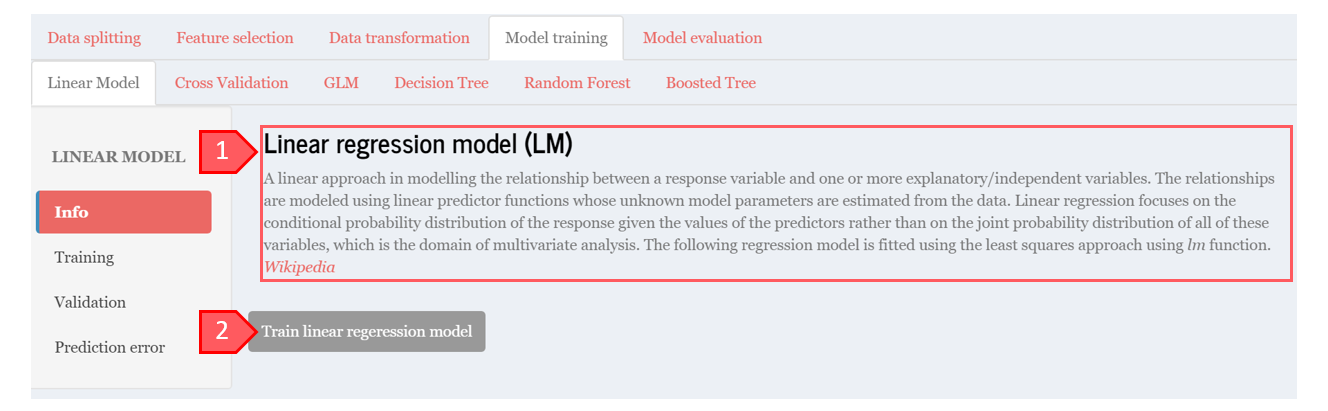
\includegraphics[width=0.95\linewidth]{images/mdltrain1} 

}

\caption{Model information page and training}\label{fig:unnamed-chunk-25}
\end{figure}

\hypertarget{b.-training-other-models}{%
\subparagraph{B. Training other models}\label{b.-training-other-models}}

Other models (Generalised Linear Model, Decision tree, Random Forest,
and Boosted Tree) require cross validation (CV) training sets. Prior to
model training, user will be required to:

{[}1{]} Navigate to the ``Cross Validation'' page

{[}2{]} Select K-fold cross validation parameter

{[}3{]} Prepare cross validation training set

\begin{figure}[H]

{\centering 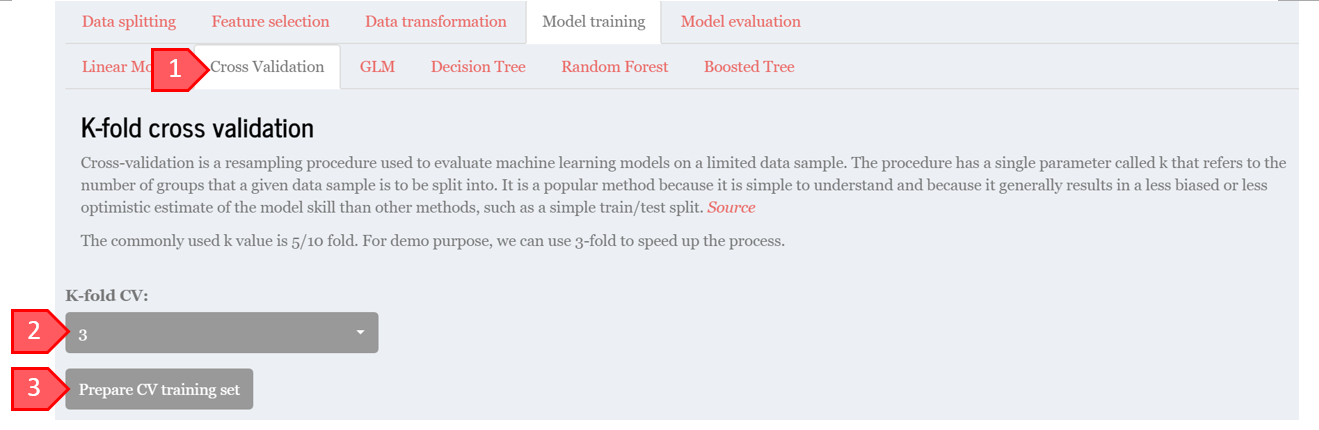
\includegraphics[width=0.95\linewidth]{images/kfold} 

}

\caption{K-fold cross validation preparation}\label{fig:unnamed-chunk-26}
\end{figure}

Once the CV training set is prepared, user can proceed to train the rest
of the models. Note that training for these models will take some time
and user will be prompted by a message which will disappear once model
training is completed.

\begin{figure}[H]

{\centering 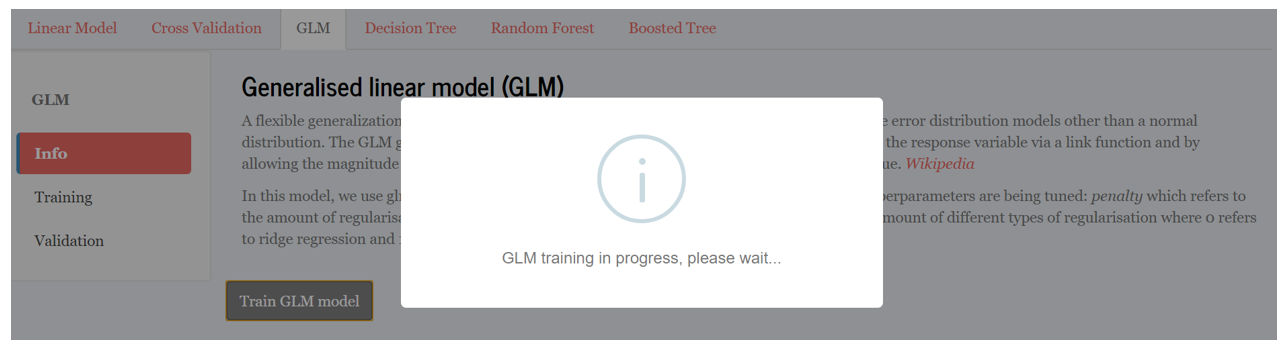
\includegraphics[width=0.95\linewidth]{images/mdltrain2} 

}

\caption{Training in progress loading page}\label{fig:unnamed-chunk-27}
\end{figure}

\hypertarget{training-result}{%
\paragraph{4.4.2 Training result}\label{training-result}}

Once model training is completed, user will be directed to the next
section for the training result.

\hypertarget{a.-linear-model}{%
\subparagraph{A. Linear model}\label{a.-linear-model}}

For linear model, the model fit result is given in a table form {[}1{]}.
Interactive exploration on coefficient estimate result is possible by
selecting p-value criteria {[}2{]}, sorting method {[}3{]}, and tooltip
information {[}4{]}. User is to proceed with model validation by
clicking on the ``Validate model'' button {[}5{]}.

\begin{figure}[H]

{\centering 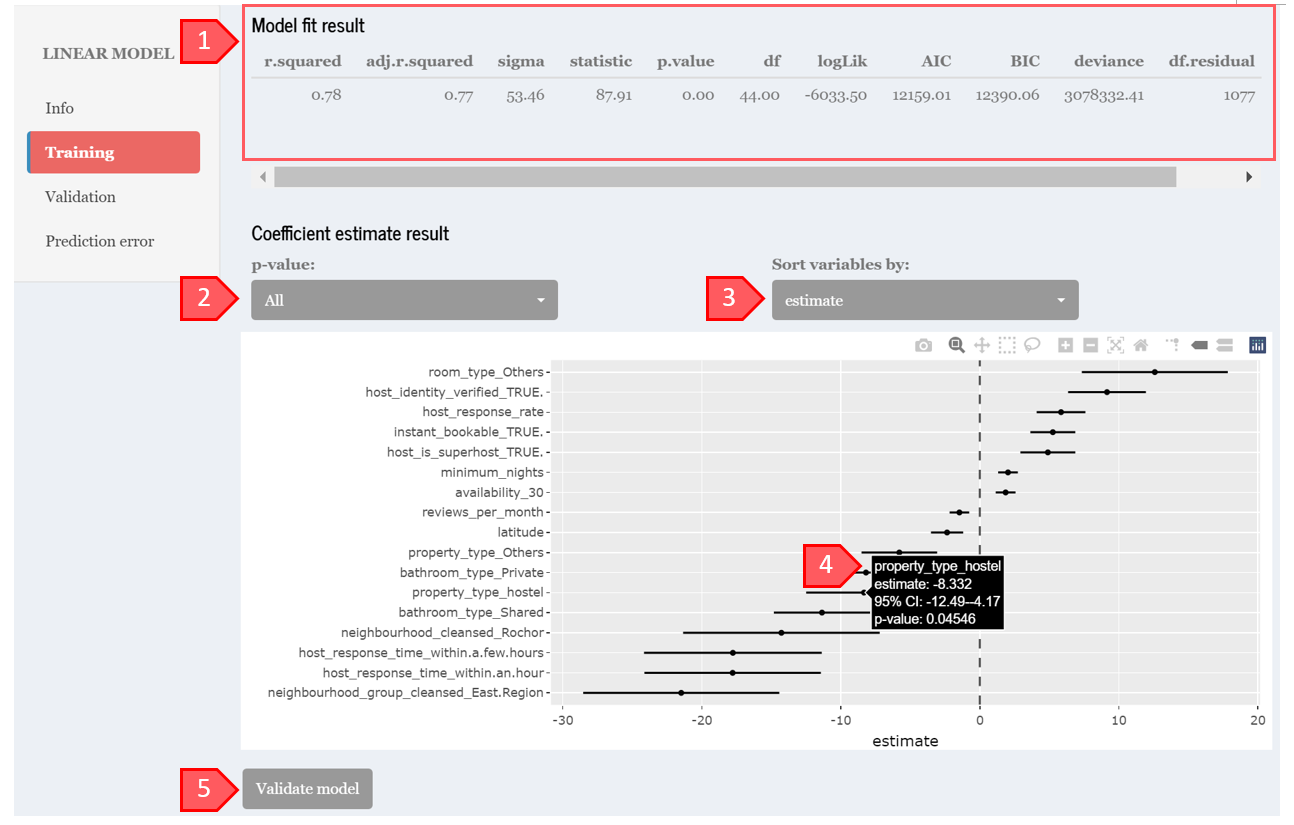
\includegraphics[width=0.95\linewidth]{images/mdltrain3} 

}

\caption{Training result page of linear model}\label{fig:unnamed-chunk-28}
\end{figure}

\hypertarget{b.-other-models}{%
\subparagraph{B. Other models}\label{b.-other-models}}

The rest of the models' training involves hyper-parameter tuning where
the summary will be displayed once training is completed.

{[}1{]} The hyper-parameters are plotted and grouped according to 4
types of metric (RMSE, MAE, MAPE, Rsquared)

{[}2{]} Next, user will be able to view the best model according to the
metric of choice through the dropdown menu selection.

{[}3{]} The data table below will respond to the metric selection and
display the best model on top

{[}4{]} Click the ``Choose best model'' button to select the best model
based on selected metric.

\begin{figure}[H]

{\centering 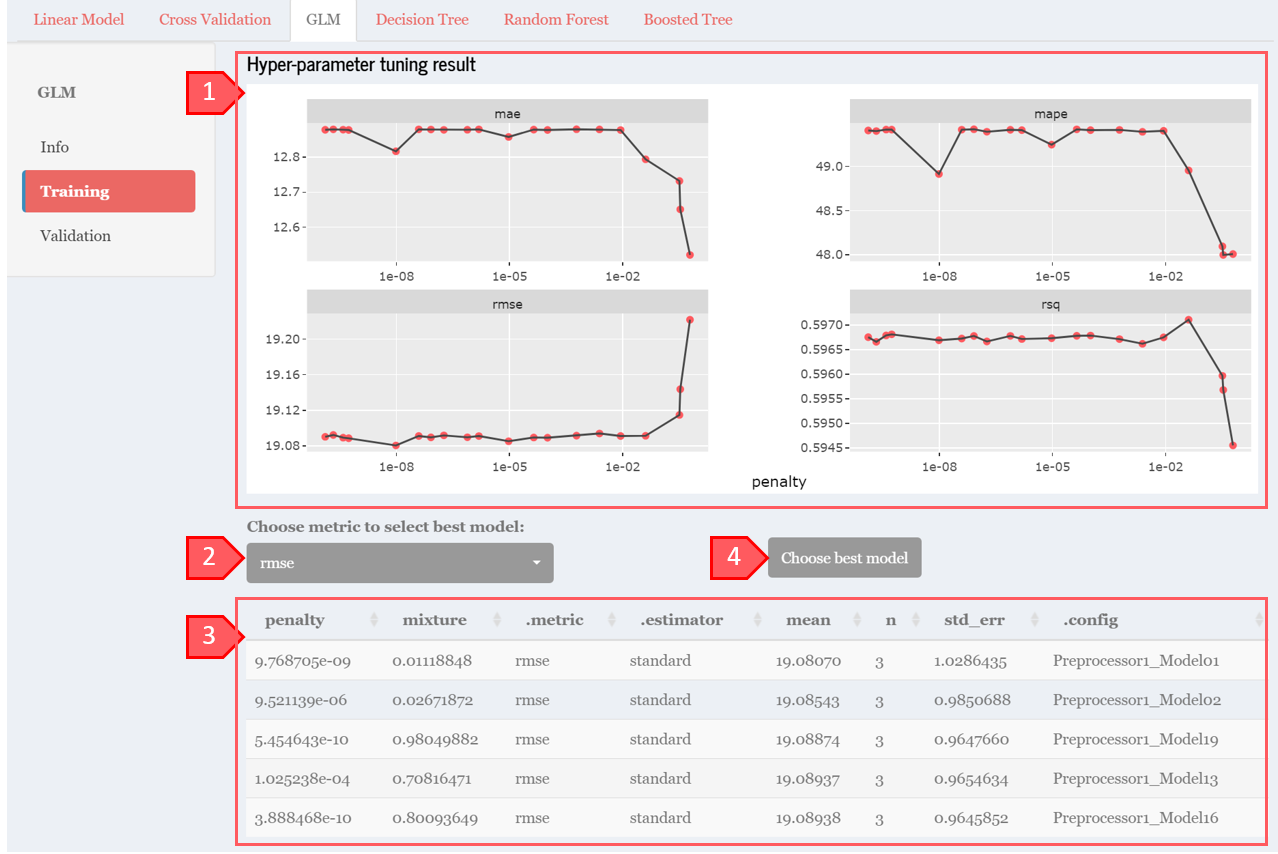
\includegraphics[width=0.95\linewidth]{images/mdltrain4} 

}

\caption{Training result page for GLM}\label{fig:unnamed-chunk-29}
\end{figure}

Once best model is selected, different information will be displayed
depending on the model algorithm. For GLM, the coefficient estimate will
be plotted and sorted according to the estimate value.

\begin{figure}[H]

{\centering 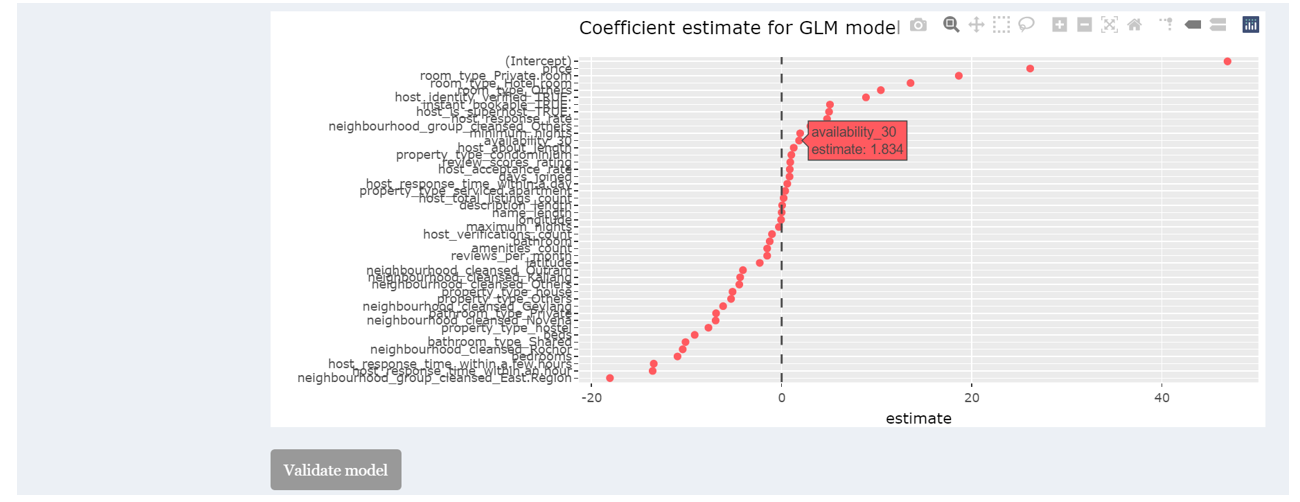
\includegraphics[width=0.95\linewidth]{images/mdltrain5} 

}

\caption{Coefficient estimate plot}\label{fig:unnamed-chunk-30}
\end{figure}

Tree based model will have variable importance score displayed, with
additional tree visualisation for decision tree model.

\begin{figure}[H]

{\centering 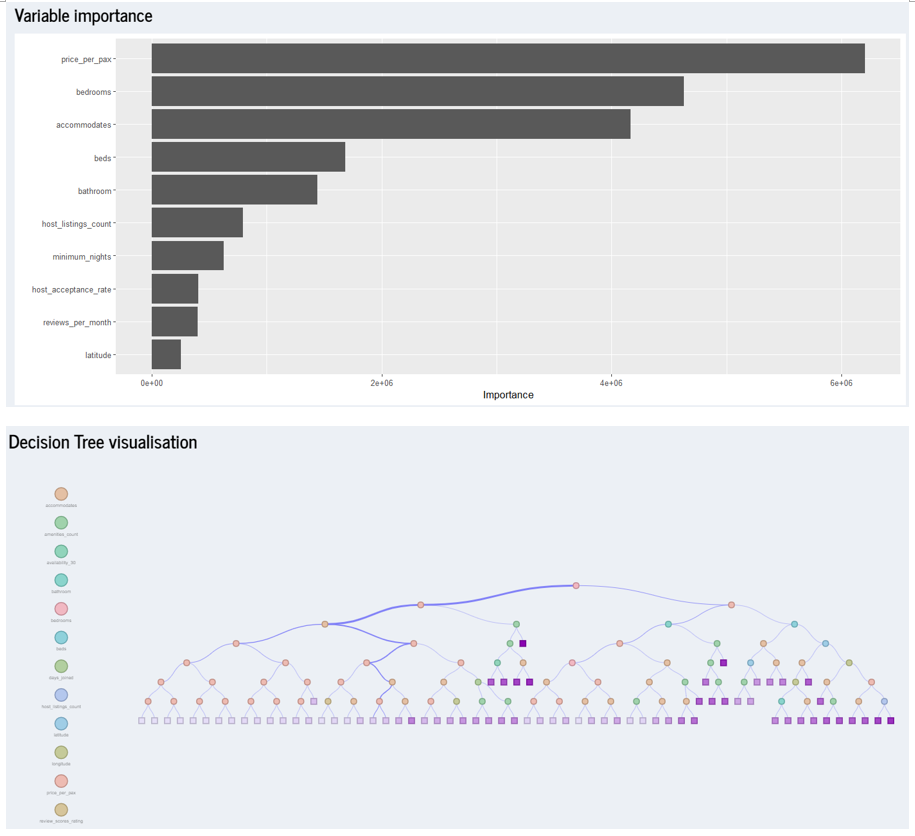
\includegraphics[width=0.95\linewidth]{images/mdltrain6} 

}

\caption{Variable importance and tree visualisation}\label{fig:unnamed-chunk-31}
\end{figure}

\hypertarget{validation-result}{%
\paragraph{4.4.3 Validation result}\label{validation-result}}

After validation process, the predicted value will be plotted against
the actual value in an Rsquare plot {[}1{]}. The calculated metric
performance is also provided below the plot {[}2{]}.

\begin{figure}[H]

{\centering 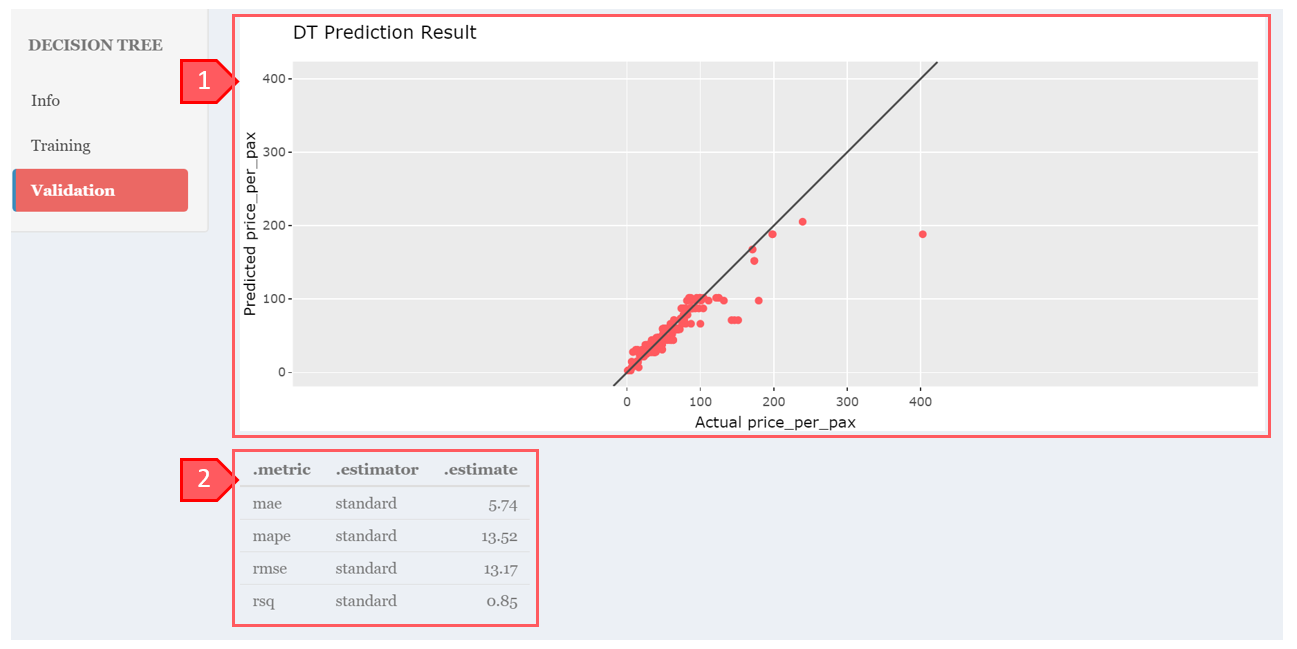
\includegraphics[width=0.95\linewidth]{images/mdltrain7} 

}

\caption{Model validation result page}\label{fig:unnamed-chunk-32}
\end{figure}

\hypertarget{prediction-error}{%
\paragraph{4.4.4 Prediction error}\label{prediction-error}}

For linear model, additional section is available to explore cases with
high prediction error.

{[}1{]} Select how many prediction points with highest deviation from
actual value

{[}2{]} Select how many top predictors to be displayed

{[}3{]} Select p-value threshold for deciding significant predictors

{[}4{]} Plot of training data distribution as histogram, overlapped with
points where prediction error is high

{[}5{]} User can single out specific point by double clicking the ``id''
number in the legend

{[}6{]} Details of point with high prediction error and their predictors
value are displayed in a table

\begin{figure}[H]

{\centering 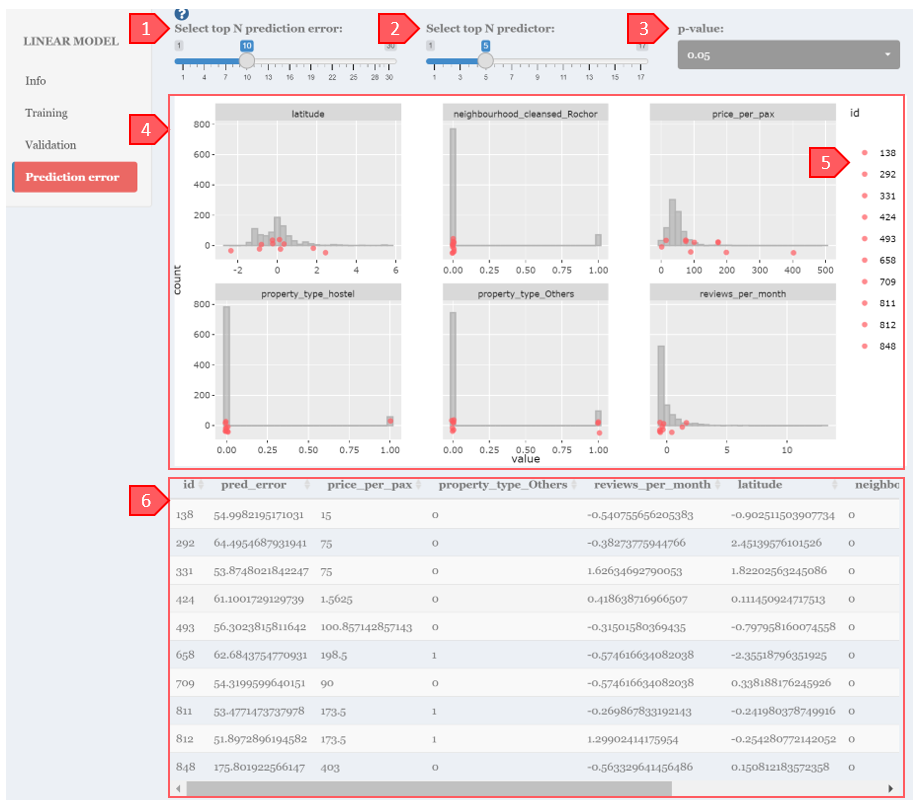
\includegraphics[width=0.95\linewidth]{images/mdltrain8} 

}

\caption{Prediction error page for further exploration}\label{fig:unnamed-chunk-33}
\end{figure}

\hypertarget{model-evaluation}{%
\subsubsection{4.5 Model evaluation}\label{model-evaluation}}

To perform model evaluation, ensure that at least 1 of the model
algorithms has been trained and validated through the previous sections.
This section comprises 3 pages:

\hypertarget{information-page}{%
\paragraph{4.5.1 Information page}\label{information-page}}

To start the evaluation, click on the ``Collect model performance''
button to gather all the best model that has been trained and validated
previously.

\begin{figure}[H]

{\centering 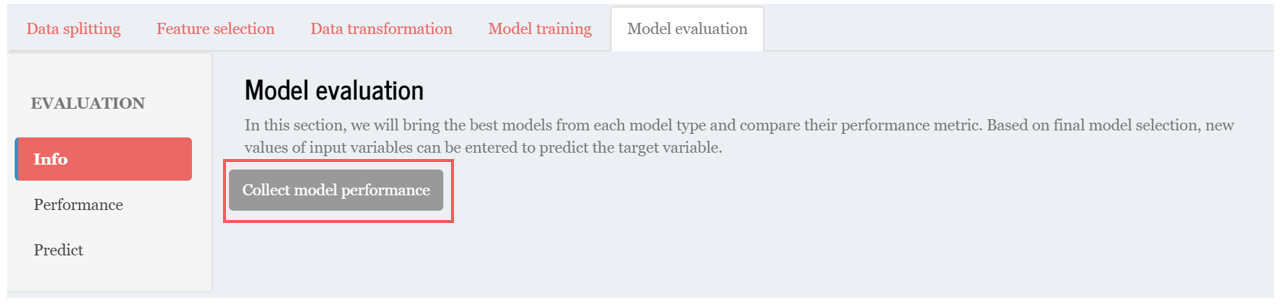
\includegraphics[width=0.95\linewidth]{images/mdleval1} 

}

\caption{Model evaluation page}\label{fig:unnamed-chunk-34}
\end{figure}

\hypertarget{performance}{%
\paragraph{4.5.2 Performance}\label{performance}}

Upon clicking the button, the next page will show:

{[}1{]} Comparison of models along with their performance metrics

{[}2{]} Through the dropdown menu, user can select the best model that
will be used for prediction

{[}3{]} Finalise model selection by clicking the button

\begin{figure}[H]

{\centering 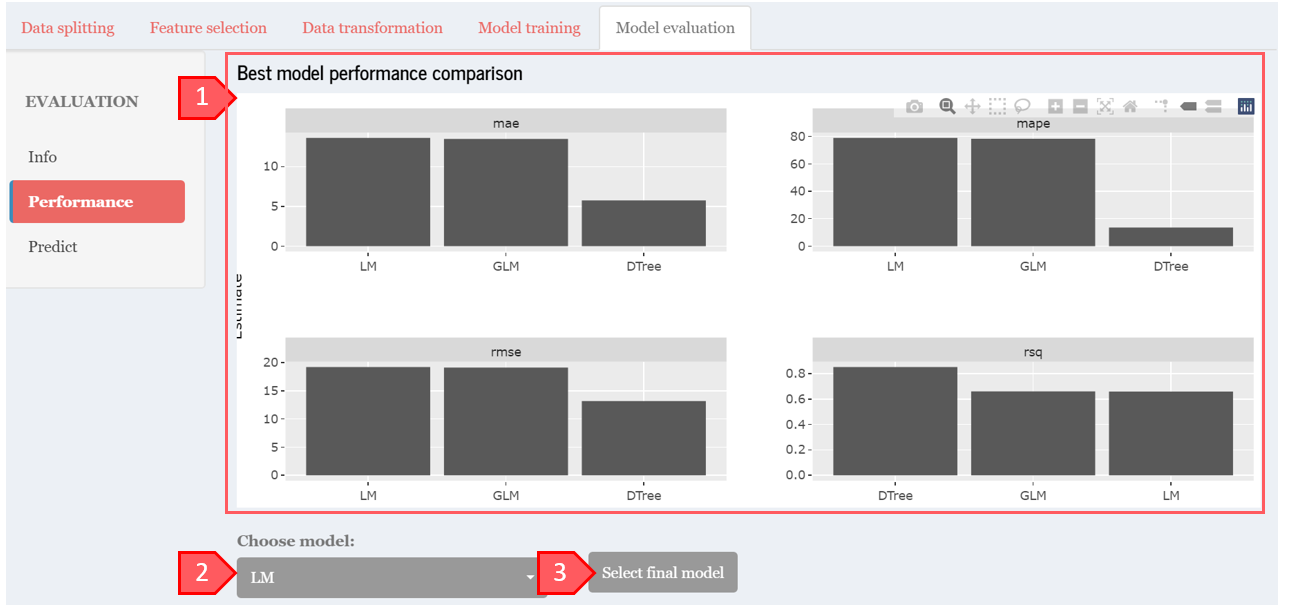
\includegraphics[width=0.95\linewidth]{images/mdleval2} 

}

\caption{Model performance comparison page}\label{fig:unnamed-chunk-35}
\end{figure}

\hypertarget{predict}{%
\paragraph{4.5.3 Predict}\label{predict}}

After selecting the final model, user will be directed to the next page
for prediction with new input variables.

{[}1{]} All variables selected for model training are displayed for user
input

{[}2{]} Once input variables are defined, click on the button to
calculate response variable using the selected model

{[}3{]} Predicted value is displayed

\begin{figure}[H]

{\centering 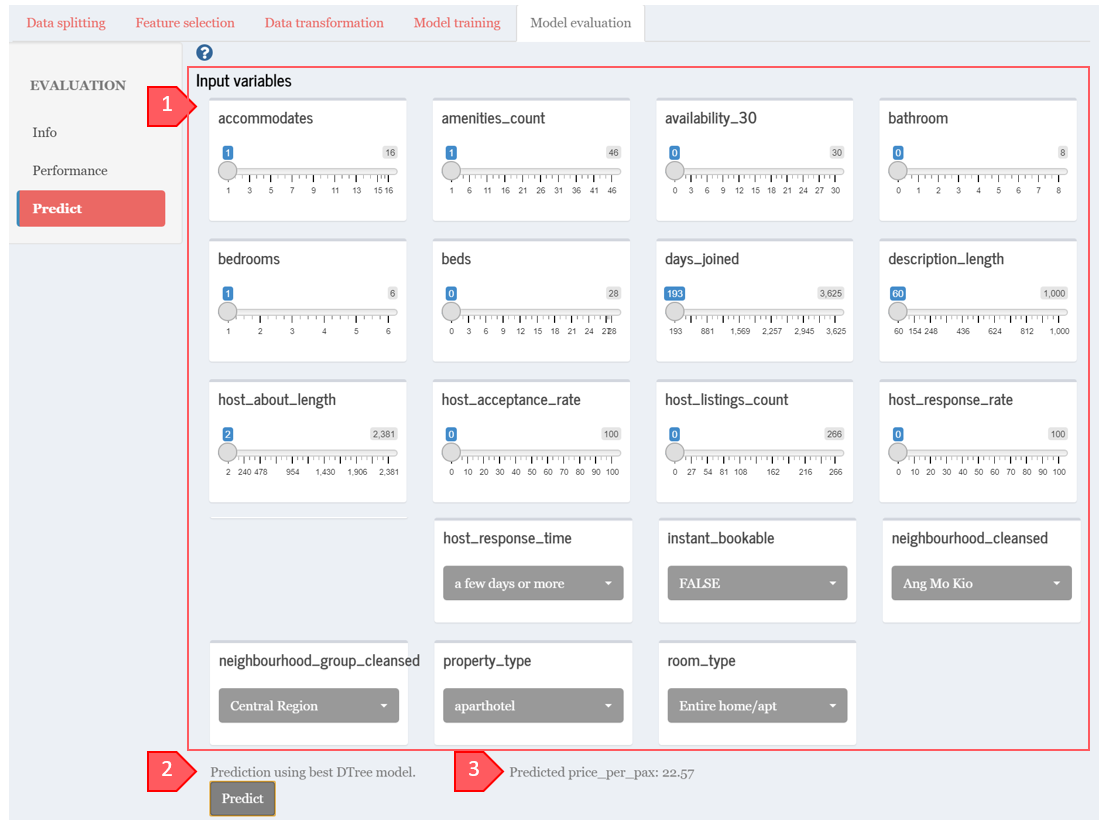
\includegraphics[width=0.95\linewidth]{images/mdleval3} 

}

\caption{Prediction page with input variables and predicted value}\label{fig:unnamed-chunk-36}
\end{figure}

\end{document}
